% This is samplepaper.tex, a sample chapter demonstrating the
% LLNCS macro package for Springer Computer Science proceedings;
% Version 2.21 of 2022/01/12
%
\documentclass[preprint,12pt,sort&compress]{elsarticle}%
\usepackage[T1]{fontenc}
% T1 fonts will be used to generate the final print and online PDFs,
% so please use T1 fonts in your manuscript whenever possible.
% Other font encondings may result in incorrect characters.
%
%\usepackage{cite}
\usepackage{listings}
\usepackage{amsmath,amssymb,amsfonts}
\usepackage{algorithmic}
\usepackage{graphicx}
\usepackage{textcomp}
\usepackage{booktabs}
\usepackage{threeparttable}
\usepackage{amsthm}
\usepackage{url}
\usepackage{makecell}
\usepackage[table]{xcolor}
\usepackage{pifont}
\usepackage{xspace}
\usepackage{float}
\usepackage{subcaption}
\usepackage{array}
\usepackage{hyperref}
\newtheorem{definition}{Definition}[section]
\newcommand{\cmark}{\ding{51}}%
\newcommand{\xmark}{\ding{55}}%
\newcommand{\amark}{\ding{107}}%
\newcommand{\lnmark}{\ding{116}}%
\newcommand{\pmark}{\ding{67}}%
\newcommand{\hmark}{\ding{168}}%
\newcommand{\missingcell}{\cellcolor{gray!25}}
\newcolumntype{R}[1]{>{\raggedleft\arraybackslash}p{#1}}
% Used for displaying a sample figure. If possible, figure files should
% be included in EPS format.
%
% If you use the hyperref package, please uncomment the following two lines
% to display URLs in blue roman font according to Springer's eBook style:
%\usepackage{color}
%\renewcommand\UrlFont{\color{blue}\rmfamily}
%
\begin{document}
%
\begin{frontmatter}

\title{Entropy Collapse in Mobile Sensors: The Hidden Risks of Sensor-Based Security}

\author[1]{Carlton Shepherd\corref{cor1}\fnref{fn1}}
\ead{carlton.shepherd@ncl.ac.uk}
\author[1]{Elliot A.\ J.\ Hurley}
\ead{e.a.j.hurley2@ncl.ac.uk}
\address[1]{School of Computing, Newcastle University, Newcastle-upon-Tyne, UK}

% Optional: Include corresponding author and footnotes if needed.
\cortext[cor1]{Corresponding author}
\fntext[fn1]{ORCID: 0000-0002-7366-9034}
%
\begin{abstract}Mobile sensor data has been proposed for security-critical applications such as device pairing, proximity detection, and continuous authentication. However, the foundational premise that these signals provide sufficient entropy remains under-explored. In this work, we systematically analyse the entropy of mobile sensor data across four diverse datasets spanning multiple application contexts. Our findings reveal pervasive biases, with single-sensor mean min-entropy values ranging from 3.408–4.483 bits ($\sigma$=1.018–1.574) despite Shannon entropy being several multiples higher, showing a significant collapse between average- to worst-case settings. We further demonstrate that correlations between sensor modalities reduce the worst-case entropy of using multiple sensors by up to $\approx$75\% compared to average-case Shannon entropy. This brings joint min-entropy well below 10 bits in many cases and, in the best case, yielding only $\approx$24 bits of min-entropy when combining 20 sensor modalities. These results raise the serious risk of attacks that exhaustively search the space of possible sensor measurements. Our work also calls into question the widely held assumption that adding more sensors inherently yields higher security, and we strongly urge caution when relying on mobile sensor data for security applications.
\end{abstract}

\begin{keyword}
Entropy \sep Sensors \sep Mobile security
\end{keyword}

\end{frontmatter}
%
%
\section{Introduction}
\label{sec:intro}

Modern mobile devices come equipped with an array of embedded sensors---accelerometers, gyroscopes, magnetometers, and others---that capture continuous motion and environmental data at fine temporal granularity. This rich sensor data has enabled applications from activity recognition to context-aware computing. More recently, research has proposed leveraging these signals for security-critical tasks such as cryptographic key generation, zero-interaction device pairing, and continuous authentication. A crucial yet under-explored assumption underpins such designs: sensor data provides sufficient unpredictability to thwart adversarial inference. Traditional ``shake-to-pair'' protocols~\cite{mayrhofer2009shake} rely on motion patterns to establish secure communication between co-located devices, while other methods have incorporated ambient phenomena, such as characteristics of magnetic fields and thermal fluctuations, to mitigate relay attacks~\cite{shrestha2014drone,shrestha2018sensor,markantonakis2024using,gurulian2017effectiveness,shepherd2017applicability} and reduce user authentication prompts~\cite{krhovjak2007sources,riva2012progressive,shi2011senguard,miettinen2014conxsense,li2013unobservable}. 

Despite these advancements, fundamental issues remain: multi-modal sensing is often advocated to counter sensor-specific weaknesses~\cite{shrestha2014drone,markantonakis2024using,truong2014comparing,mehrnezhad2015tap}, but the quantitative security benefits of combining multiple sensors has not been rigorously evaluated. Many existing studies rely on heuristic assessments or machine learning classifiers, e.g.~\cite{markantonakis2024using,mehrnezhad2015tap,gurulian2018good,shrestha2014drone,truong2014comparing}, that do not address critical security questions. That is, firstly, how much entropy do sensors truly provide? And, secondly, to what extent do multi-modal sensor combinations provide security gains? Understanding the \emph{underlying} entropy is important: even if different sensors are combined, fused or otherwise transformed, it does \emph{not} fundamentally improve the quantity of entropy, or unpredictability, inherent in such signals. This paper investigates those concerns.

Our analysis reveals systemic limitations: commodity sensors exhibit significant biases of between 3.408--4.483 bits of min-entropy (5.584--9.266 bits of Shannon entropy on average). In this paper, we analyse 25 different sensors compared to a far smaller number explored in related work, i.e.\ \cite{voris2011accelerometers} (1 sensor), \cite{hennebert2013entropy} (10), \cite{krhovjak2007sources} (2), and \cite{lv2020analysis} (3). Furthermore, to the best of our knowledge, we also present the first multi-modal entropy analysis at this scale. We find that, while multi-modal sensor usage confers some benefits, non-uniform distributions and inter-sensor correlations significantly reduce the worst-case min-entropy by $\approx$40--75\% compared to average-case Shannon entropy. These findings challenge the notion that increasing the number of sensors reliably strengthens security, and it underscores the inadequacy of using sensor data as a dependable entropy source. Our contributions are as follows:
\begin{itemize} 
\item We introduce the first systematic approach to evaluating sensor entropy across such a comprehensive range of modalities and datasets using various entropy metrics (max, Shannon, collision, and min-entropy).
\item We empirically demonstrate how inter-sensor correlations and biases erode entropy, casting doubt on the proposition that using multiple sensors adds substantially to security. 
\item We show how the collapse in worst-case entropy opens the door to attacks that exhaustively enumerate, or brute force, the (joint) measurement space. This gives rise to fundamental security risks to schemes that rely on signals from single and multiple mobile sensors.
\item Ultimately, we advise against relying on commodity sensors as sources of unpredictability for security-critical applications, both on a single- and multiple-sensor basis.
\end{itemize}

The rest of this paper is organised in the following way: \S\ref{sec:background} discusses sensor-based security mechanisms and established entropy metrics. \S\ref{sec:design} explains our experiment design for entropy estimation, including the threat model and dataset selection. \S\ref{sec:entropy-analysis} presents empirical results of our analyses and \S\ref{sec:security-evaluation} discusses the implications for system design. We conclude in \S\ref{sec:conc} with recommendations for further work. Our analysis work is released publicly to foster future research.\footnote{\url{https://github.com/cgshep/entropy-collapse-mobile-sensors}}

\section{Background}\label{sec:backgrnd}

\subsection{Cold Start Latency and Mitigation Techniques}

Traditional FaaS platforms mitigate cold starts through snapshotting, lightweight virtualization, and warm-state management. Snapshot-based methods like \textbf{REAP} and \textbf{Catalyzer} reduce initialization time by preloading or restoring container states but require significant memory and I/O resources, limiting scalability~\cite{dong_catalyzer_2020, ustiugov_benchmarking_2021}. Lightweight virtualization solutions, such as \textbf{Firecracker} microVMs, achieve fast startup times with strong isolation but depend on robust infrastructure, making them less adaptable to fluctuating workloads~\cite{agache_firecracker_2020}. Warm-state management techniques like \textbf{Faa\$T}~\cite{romero_faa_2021} and \textbf{Kraken}~\cite{vivek_kraken_2021} keep frequently invoked containers ready, balancing readiness and cost efficiency under predictable workloads but incurring overhead when demand is erratic~\cite{romero_faa_2021, vivek_kraken_2021}. While these methods perform well in resource-rich cloud environments, their resource intensity challenges applicability in edge settings.

\subsubsection{Edge FaaS Perspective}

In edge environments, cold start mitigation emphasizes lightweight designs, resource sharing, and hybrid task distribution. Lightweight execution environments like unikernels~\cite{edward_sock_2018} and \textbf{Firecracker}~\cite{agache_firecracker_2020}, as used by \textbf{TinyFaaS}~\cite{pfandzelter_tinyfaas_2020}, minimize resource usage and initialization delays but require careful orchestration to avoid resource contention. Function co-location, demonstrated by \textbf{Photons}~\cite{v_dukic_photons_2020}, reduces redundant initializations by sharing runtime resources among related functions, though this complicates isolation in multi-tenant setups~\cite{v_dukic_photons_2020}. Hybrid offloading frameworks like \textbf{GeoFaaS}~\cite{malekabbasi_geofaas_2024} balance edge-cloud workloads by offloading latency-tolerant tasks to the cloud and reserving edge resources for real-time operations, requiring reliable connectivity and efficient task management. These edge-specific strategies address cold starts effectively but introduce challenges in scalability and orchestration.

\subsection{Predictive Scaling and Caching Techniques}

Efficient resource allocation is vital for maintaining low latency and high availability in serverless platforms. Predictive scaling and caching techniques dynamically provision resources and reduce cold start latency by leveraging workload prediction and state retention.
Traditional FaaS platforms use predictive scaling and caching to optimize resources, employing techniques (OFC, FaasCache) to reduce cold starts. However, these methods rely on centralized orchestration and workload predictability, limiting their effectiveness in dynamic, resource-constrained edge environments.



\subsubsection{Edge FaaS Perspective}

Edge FaaS platforms adapt predictive scaling and caching techniques to constrain resources and heterogeneous environments. \textbf{EDGE-Cache}~\cite{kim_delay-aware_2022} uses traffic profiling to selectively retain high-priority functions, reducing memory overhead while maintaining readiness for frequent requests. Hybrid frameworks like \textbf{GeoFaaS}~\cite{malekabbasi_geofaas_2024} implement distributed caching to balance resources between edge and cloud nodes, enabling low-latency processing for critical tasks while offloading less critical workloads. Machine learning methods, such as clustering-based workload predictors~\cite{gao_machine_2020} and GRU-based models~\cite{guo_applying_2018}, enhance resource provisioning in edge systems by efficiently forecasting workload spikes. These innovations effectively address cold start challenges in edge environments, though their dependency on accurate predictions and robust orchestration poses scalability challenges.

\subsection{Decentralized Orchestration, Function Placement, and Scheduling}

Efficient orchestration in serverless platforms involves workload distribution, resource optimization, and performance assurance. While traditional FaaS platforms rely on centralized control, edge environments require decentralized and adaptive strategies to address unique challenges such as resource constraints and heterogeneous hardware.



\subsubsection{Edge FaaS Perspective}

Edge FaaS platforms adopt decentralized and adaptive orchestration frameworks to meet the demands of resource-constrained environments. Systems like \textbf{Wukong} distribute scheduling across edge nodes, enhancing data locality and scalability while reducing network latency. Lightweight frameworks such as \textbf{OpenWhisk Lite}~\cite{kravchenko_kpavelopenwhisk-light_2024} optimize resource allocation by decentralizing scheduling policies, minimizing cold starts and latency in edge setups~\cite{benjamin_wukong_2020}. Hybrid solutions like \textbf{OpenFaaS}~\cite{noauthor_openfaasfaas_2024} and \textbf{EdgeMatrix}~\cite{shen_edgematrix_2023} combine edge-cloud orchestration to balance resource utilization, retaining latency-sensitive functions at the edge while offloading non-critical workloads to the cloud. While these approaches improve flexibility, they face challenges in maintaining coordination and ensuring consistent performance across distributed nodes.


\newcommand{\tabincell}[2]{\begin{tabular}{@{}#1@{}}#2\end{tabular}}
\newcommand{\rowstyle}[1]{\gdef\currentrowstyle{#1}%
	#1\ignorespaces
}

\newcommand{\className}[1]{\textbf{\sf #1}}
\newcommand{\functionName}[1]{\textbf{\sf #1}}
\newcommand{\objectName}[1]{\textbf{\sf #1}}
\newcommand{\annotation}[1]{\textbf{#1}}
\newcommand{\todo}[1]{\textcolor{blue}{\textbf{[[TODO: #1]]}}}
\newcommand{\change}[1]{\textcolor{blue}{#1}}
\newcommand{\fetch}[1]{\textbf{\em #1}}
\newcommand{\phead}[1]{\vspace{1mm} \noindent {\bf #1}}
\newcommand{\wei}[1]{\textcolor{blue}{{\it [Wei says: #1]}}}
\newcommand{\peter}[1]{\textcolor{red}{{\it [Peter says: #1]}}}
\newcommand{\zhenhao}[1]{\textcolor{dkblue}{{\it [Zhenhao says: #1]}}}
\newcommand{\feng}[1]{\textcolor{magenta}{{\it [Feng says: #1]}}}
\newcommand{\jinqiu}[1]{\textcolor{red}{{\it [Jinqiu says: #1]}}}
\newcommand{\shouvick}[1]{\textcolor{violet(ryb)}{{\it [Shouvick says: #1]}}}
\newcommand{\pattern}[1]{\emph{#1}}
%\newcommand{\tool}{{{DectGUILag}}\xspace}
\newcommand{\tool}{{{GUIWatcher}}\xspace}


\newcommand{\guo}[1]{\textcolor{yellow}{{\it [Linqiang says: #1]}}}

\newcommand{\rqbox}[1]{\begin{tcolorbox}[left=4pt,right=4pt,top=4pt,bottom=4pt,colback=gray!5,colframe=gray!40!black,before skip=2pt,after skip=2pt]#1\end{tcolorbox}}

To begin with, we sought publicly available sensor datasets suitable for analysing motion and environmental data at scale. Our search involved broad queries across IEEE DataPort, Google Scholar, Google Dataset Search, and GitHub. Several ostensibly ``open'' datasets either were no longer downloadable or imposed restrictive licensing terms~\cite{Mahbub_Btas2016_UMDAA02,stragapede2023behavepassdb,acien2021becaptcha}. Ultimately, we narrowed our scope to four datasets that offer diverse usage contexts, consistent sampling rates, and documented sensor modalities:

\begin{itemize}
    \item \emph{UCI-HAR}~\cite{anguita2013public}:  A widely referenced dataset for human activity recognition, comprising smartphone sensor recordings from multiple subjects performing daily activities. Data includes triaxial accelerometer and gyroscope signals.

    
    \item \emph{University of Sussex--Huawei Locomotion (SHL)}~\cite{gjoreski2018university,wang2019enabling}:   sampled at 100 Hz from an Huawei Mate 9 smartphone. The publicly available SHL Preview dataset is used, comprising three recording-days per user (59 hours of data in total). To scope this study, we use the dataset from the handheld mobile phone as a good fit with related work.
    \item \emph{Relay}~\cite{gurulian2017effectiveness}: Contains sensor measurements for approximately 1{,}500 NFC-based contactless transactions, each recorded at 100\,Hz across several physical locations (e.g., caf\'{e}s). The dataset encompasses accelerometer, gyroscope, and environmental readings taken in realistic payment scenarios.
    \item \emph{PerilZIS}~\cite{fomichev2019perils}: Collected at 10\,Hz from a Texas Instruments SensorTag, a Samsung Galaxy S6, and a Samsung Galaxy Gear, this dataset spans multiple zero-interaction security use cases in an office environment.
\end{itemize}

These four datasets provide a variety of sensor types, user activities, and sampling rates, allowing us to explore how intrinsic biases and correlations manifest across different scenarios. Next, we detail how we preprocess and aggregate this data to form global distributions for our entropy analyses.
\section{Entropy Analysis}
\label{sec:entropy-analysis}

In this section, we analyse the intrinsic entropy of sensor data under the threat model described in \S\ref{sec:design}. We begin by discussing the challenges in quantising naturally continuous sensor values for discrete-entropy calculations, then present our findings for our single- and multi-sensor analyses.

\subsection{Pre-processing}

A crucial, yet underexplored, issue in prior work (e.g.\ \cite{voris2011accelerometers,lv2020analysis,hennebert2013entropy,mai2017guessability}) is how to convert inherently continuous sensor outputs into suitable discrete values for entropy estimation. For example, Shannon and min-entropy, as defined in Eqs.~\ref{eq:renyi_H1} and \ref{eq:renyi_Hinf}, rely on discrete random variables. Physical quantities such as linear acceleration or angular velocity are continuous in nature, even though modern sensors employ internal analog-to-digital conversion with a finite resolution. Yet, a sensor's advertised resolution (e.g.\ 12 bits for the widely used Bosch BMA mobile accelerometer~\cite{bosch_bma400}) does \emph{not} imply uniform coverage across its range. Everyday usage introduces biases and clustering, resulting in some measurements occurring far more frequently than others. For instance, \emph{UCI-HAR} data shows accelerometer readings concentrated in certain areas, and approximately 60\% of gyroscope readings hover near zero (see Figure~\ref{fig:acc-cdfs}). Such skew and bias radically diminishes entropy compared to uniformly distributed values.

\begin{figure*}
    \centering
    \begin{subfigure}[t]{0.333\textwidth}
        \centering
        \includegraphics[width=\textwidth]{figures/graphs/acc_x_cdf.pdf}
        \caption{Acc.\ $x$ axis.}
        \label{subfig:acx}
    \end{subfigure}%
    \begin{subfigure}[t]{0.333\textwidth}
        \centering
        \includegraphics[width=\textwidth]{figures/graphs/acc_y_cdf.pdf}
        \caption{Acc.\ $y$ axis.}
        \label{subfig:acy}
    \end{subfigure}%
    \begin{subfigure}[t]{0.333\textwidth}
        \centering
        \includegraphics[width=\textwidth]{figures/graphs/acc_z_cdf.pdf}
        \caption{Acc.\ $z$ axis.}
        \label{subfig:acz}
    \end{subfigure}

    \begin{subfigure}[t]{0.333\textwidth}
        \centering
        \includegraphics[width=\textwidth]{figures/graphs/gyro_x_cdf.pdf}
        \caption{Gyro.\ $x$ axis.}
        \label{subfig:gyx}
    \end{subfigure}%
    \begin{subfigure}[t]{0.333\textwidth}
        \centering
        \includegraphics[width=\textwidth]{figures/graphs/gyro_y_cdf.pdf}
        \caption{Gyro.\ $y$ axis.}
        \label{subfig:gyy}
    \end{subfigure}%
    \begin{subfigure}[t]{0.333\textwidth}
        \centering
        \includegraphics[width=\textwidth]{figures/graphs/gyro_z_cdf.pdf}
        \caption{Gyro.\ $z$ axis.}
        \label{subfig:gyz}
    \end{subfigure}

    \begin{subfigure}[t]{0.333\textwidth}
        \centering
        \includegraphics[width=\textwidth]{figures/graphs/Accelerometer_cdf.pdf}
        \caption{Accelerometer.}
        \label{subfig:acc}
    \end{subfigure}%
    \begin{subfigure}[t]{0.333\textwidth}
        \centering
        \includegraphics[width=\textwidth]{figures/graphs/Gyroscope_cdf.pdf}
        \caption{Gyroscope.}
        \label{subfig:gyro}
    \end{subfigure}%
    \begin{subfigure}[t]{0.333\textwidth}
        \centering
        \includegraphics[width=\textwidth]{figures/graphs/Light_cdf.pdf}
        \caption{Light.}
        \label{subfig:light}
    \end{subfigure}

    \begin{subfigure}[t]{0.333\textwidth}
        \centering
        \includegraphics[width=\textwidth]{figures/graphs/LinearAcceleration_cdf.pdf}
        \caption{Linear Acceleration.}
        \label{subfig:linacc}
    \end{subfigure}%
    \begin{subfigure}[t]{0.333\textwidth}
        \centering
        \includegraphics[width=\textwidth]{figures/graphs/MagneticField_cdf.pdf}
        \caption{Magnetometer.}
        \label{subfig:mag}
    \end{subfigure}%
    \begin{subfigure}[t]{0.333\textwidth}
        \centering
        \includegraphics[width=\textwidth]{figures/graphs/RotationVector_cdf.pdf}
        \caption{Rotation Vector.}
        \label{subfig:rv}
    \end{subfigure}
    \caption{Global sensor data CDFs -- UCI-HAR (a--f) and Relay (g--l) datasets.}
    \label{fig:acc-cdfs}
\end{figure*}

Another practical challenge arises when extremely fine-grained values appear infrequently or with negligible probability in reality. Treating every minute fluctuation (e.g.\ 9.001$ms^{-2}$ vs.\ 9.002$ms^{-2}$ for an accelerometer) as distinct outcomes can also artificially inflate entropy estimates.  In real-world applications, it is the `similarity' between measurement signals that is considered useful in existing work. It would be extremely difficult for users to reliably reproduce high-precision movements capable of effectively utilising a sensor's digital resolution (say at 0.001ms$^{-2}$ for an accelerometer). To address this, we discretise the data values into bins of similar value. However, this raises a further question of what constitutes a good strategy for selecting the number of bins and their widths? Several techniques exist that make assumptions about the underlying distribution, e.g.\ Gaussian; have different computational complexities; and are robust to outliers and data variability. To this end, we use the Freedman-Diaconis method, a commonly used robust estimator that accounts for data size and its variability.\footnote{Alternatively, a binning strategy could be employed that reflects how precisely humans can realistically replicate sensor-input changes. We defer this to future research.} This is calculated in Eq.~\ref{sec:freedman}, where $IQR(x)$ represents the interquartile range of $x$ and $n$ is the total number of samples.


\begin{equation}
    h = 2 \cdot \frac{IQR(x)}{n^{1/3}}
    \label{sec:freedman}
\end{equation}


\subsection{Single Sensors}



\begin{table}
\renewcommand{\arraystretch}{2}
\centering
\caption{Single-sensor entropy values (in bits) for each dataset. Grey cells denote unavailable data for that dataset and modality.}
\resizebox{\linewidth}{!}{%
\label{tab:single-sensor-results}
\small
\begin{tabular}{@{}r|ccc|c|ccc|c|ccc|c|ccc|c@{}}
\toprule
 & \multicolumn{16}{c}{\textbf{Dataset}} \\
 & \multicolumn{4}{c|}{\textbf{UCI-HAR}} 
 & \multicolumn{4}{c|}{\textbf{SHL}}  
 & \multicolumn{4}{c|}{\textbf{Relay}*}  
 & \multicolumn{4}{c}{\textbf{PerilZIS}} \\
\midrule
\textbf{Sensor} 
 & \(H_{0}\) & \(H_{1}\) & \(H_{2}\) & \(H_{\infty}\) 
 & \(H_{0}\) & \(H_{1}\) & \(H_{2}\) & \(H_{\infty}\) 
 & \(H_{0}\) & \(H_{1}\) & \(H_{2}\) & \(H_{\infty}\) 
 & \(H_{0}\) & \(H_{1}\) & \(H_{2}\) & \(H_{\infty}\) \\
\midrule
Acc.X       
 & 8.488 & 7.080 & 5.876 & 3.729 
 & 11.557 & 8.732  & 7.487  & 4.543 
 & \missingcell & \missingcell & \missingcell & \missingcell 
 & 13.012 & 9.292  & 6.359  & 3.626 \\
Acc.Y       
 & 8.243 & 7.231 & 6.847 & 5.694 
 & 11.425 & 8.928  & 7.717  & 4.500 
 & \missingcell & \missingcell & \missingcell & \missingcell 
 & 9.549  & 5.873  & 4.483  & 2.889 \\
Acc.Z       
 & 8.455 & 7.397 & 7.069 & 6.020 
 & 10.428 & 7.627  & 6.366  & 3.785 
 & \missingcell & \missingcell & \missingcell & \missingcell 
 & 9.817  & 6.671  & 5.403  & 4.002 \\
Acc.Mag    
 & 8.895 & 6.284 & 4.819 & 3.489 
 & 14.583 & 10.136 & 8.710  & 6.435 
 & 10.145 & 6.843 & 5.808 & 4.538
 & 13.328 & 8.273  & 7.115  & 4.526 \\
\midrule
Gyro.X     
 & 8.683 & 5.430 & 3.504 & 1.929 
 & 15.024 & 10.532 & 8.107  & 4.993 
 & \missingcell & \missingcell & \missingcell & \missingcell 
 & 14.528 & 7.231  & 4.454  & 2.805 \\
Gyro.Y     
 & 8.439 & 5.023 & 3.461 & 2.300 
 & 15.085 & 10.283 & 7.601  & 4.827 
 & \missingcell & \missingcell & \missingcell & \missingcell 
 & 14.078 & 6.715  & 4.039  & 2.529 \\
Gyro.Z     
 & 8.714 & 5.675 & 3.948 & 2.363 
 & 15.281 & 10.070 & 5.708  & 3.083 
 & \missingcell & \missingcell & \missingcell & \missingcell 
 & 13.961 & 6.463  & 3.836  & 2.434 \\
Gyro.Mag  
 & 8.414 & 5.759 & 4.130 & 2.537 
 & 12.123 & 7.816  & 5.728  & 3.699 
 & 7.954 & 4.751 & 3.442 & 2.083 
 & 14.166 & 5.565  & 1.932  & 0.969 \\
\midrule
Mag.X   
 & \missingcell & \missingcell & \missingcell & \missingcell 
 & 12.845 & 8.840  & 8.386  & 6.374 
 & \missingcell & \missingcell & \missingcell & \missingcell 
 & 10.767 & 7.639  & 6.816  & 4.883 \\
Mag.Y   
 & \missingcell & \missingcell & \missingcell & \missingcell 
 & 12.263 & 8.737  & 8.314  & 6.223 
 & \missingcell & \missingcell & \missingcell & \missingcell 
 & 10.179 & 7.622  & 6.605  & 4.405 \\
Mag.Z   
 & \missingcell & \missingcell & \missingcell & \missingcell 
 & 12.516 & 8.586  & 8.217  & 6.228 
 & \missingcell & \missingcell & \missingcell & \missingcell 
 & 10.129 & 7.507  & 6.726  & 4.448 \\
Mag.Mag 
 & \missingcell & \missingcell & \missingcell & \missingcell 
 & 13.558 & 9.436  & 8.771  & 7.148 
 & 7.972 & 6.147 & 5.617 & 4.254
 & 10.293 & 7.329  & 6.489  & 4.454 \\
\midrule
Rot.\ Vec.\ 
 & \missingcell & \missingcell & \missingcell & \missingcell 
 & 8.725  & 7.721  & 5.970  & 3.220 
 & 5.000 & 3.307 & 1.965 & 1.021
 & \missingcell & \missingcell & \missingcell & \missingcell \\
\midrule
Grav.X     
 & \missingcell & \missingcell & \missingcell & \missingcell 
 & 9.014  & 8.482  & 7.266  & 4.299 
 & \missingcell & \missingcell & \missingcell & \missingcell 
 & \missingcell & \missingcell & \missingcell & \missingcell \\
Grav.Y     
 & \missingcell & \missingcell & \missingcell & \missingcell 
 & 9.338  & 8.770  & 7.602  & 4.453 
 & \missingcell & \missingcell & \missingcell & \missingcell 
 & \missingcell & \missingcell & \missingcell & \missingcell \\
Grav.Z     
 & \missingcell & \missingcell & \missingcell & \missingcell 
 & 8.180  & 7.193  & 5.418  & 3.036 
 & \missingcell & \missingcell & \missingcell & \missingcell 
 & \missingcell & \missingcell & \missingcell & \missingcell \\
Grav.Mag     
 & \missingcell & \missingcell & \missingcell & \missingcell 
 & 14.373 & 7.988  & 7.227  & 6.242 
 & 7.794 & 6.325 & 5.864 & 4.532
 & \missingcell & \missingcell & \missingcell & \missingcell \\
\midrule
LinAcc.X  
 & \missingcell & \missingcell & \missingcell & \missingcell 
 & 15.260 & 10.077 & 7.621  & 5.116 
 & \missingcell & \missingcell & \missingcell & \missingcell 
 & \missingcell & \missingcell & \missingcell & \missingcell \\
LinAcc.Y  
 & \missingcell & \missingcell & \missingcell & \missingcell 
 & 14.859 & 10.116 & 7.639  & 5.224 
 & \missingcell & \missingcell & \missingcell & \missingcell 
 & \missingcell & \missingcell & \missingcell & \missingcell \\
LinAcc.Z  
 & \missingcell & \missingcell & \missingcell & \missingcell 
 & 14.377 & 9.951  & 7.605  & 4.543 
 & \missingcell & \missingcell & \missingcell & \missingcell 
 & \missingcell & \missingcell & \missingcell & \missingcell \\
LinAcc.Mag  
 & \missingcell & \missingcell & \missingcell & \missingcell 
 & 12.777 & 7.968  & 5.752  & 3.420 
 & 9.175 & 6.385 & 5.424 & 4.222
 & \missingcell & \missingcell & \missingcell & \missingcell \\
\midrule
Light       
 & \missingcell & \missingcell & \missingcell & \missingcell 
 & \missingcell & \missingcell & \missingcell & \missingcell 
 & 7.200& 5.331 & 4.507& 3.206
 & 12.152 & 7.940  & 7.137  & 4.552 \\
Humidity    
 & \missingcell & \missingcell & \missingcell & \missingcell 
 & \missingcell & \missingcell & \missingcell & \missingcell 
 & \missingcell & \missingcell & \missingcell & \missingcell 
 & 7.943  & 7.048  & 6.774  & 5.546 \\
Temp.       
 & \missingcell & \missingcell & \missingcell & \missingcell 
 & 7.295  & 4.753  & 2.611  & 1.332 
 & \missingcell & \missingcell & \missingcell & \missingcell 
 & 8.484  & 7.416  & 6.941  & 5.449 \\
Pressure    
 & \missingcell & \missingcell & \missingcell & \missingcell 
 & 9.461  & 8.170  & 7.723  & 6.237 
 & \missingcell & \missingcell & \missingcell & \missingcell 
 & 8.044  & 7.006  & 6.370  & 5.073 \\
\midrule 
\textbf{Mean} 
 & 8.541 & 6.235 & 4.957 & 3.508 
 & 13.188 & 9.266 & 7.178 & 4.483 
 & 7.891 & 5.584 & 4.661 & 3.408 
 & 11.277 & 7.224 & 5.717 & 3.912 \\
\textbf{S.D.} 
 & 0.207 & 0.904 & 1.461 & 1.574 
 & 1.993 & 1.148 & 1.115 & 1.018 
 & 1.612 & 1.227 & 1.474 & 1.379 
 & 2.312 & 0.900 & 1.526 & 1.266 \\\bottomrule
\end{tabular}
}
\end{table}


Given the biases discussed above, it is inevitable that some sensor readings will exhibit relatively high predictability. To quantify this, we calculate individual-sensor entropies across multiple datasets. The results are given in Table~\ref{tab:single-sensor-results}. For multi-dimensional modalities (e.g.\ triaxial accelerometer or gyroscope), these are split into separate axes following Voris et al.~\cite{voris2011accelerometers}. We note that, in the Relay dataset, the data for individual $x$, $y$ and $z$ components are not given for the accelerometer, gyroscope, and magnetometer sensors. Rather, the authors have already preprocessed triaxial data into its vector magnitudes, i.e.\ $\textbf{v} = \sqrt{x^2 + y^2 + z^2}$. We give this as ``X.Mag'' for a given sensor X. For completeness, we compute the magnitude ourselves for other datasets, where applicable, and report the entropy values for this new synthetic modality.

Several clear patterns emerge from Table~\ref{tab:single-sensor-results}. Some sensors, such as certain accelerometer axes in \emph{SHL} or \emph{PerilZIS}, exhibit moderate min-entropies of 4--6 bits. Other sensors, particularly gyroscope axes (see \emph{UCI-HAR}) show values below 3 bits, indicating high predictability in their most frequent readings. Shannon entropy values (\(H_1\)) can be fairly high (up to 10 bits in some cases), whereas min-entropy (\(H_{\infty}\)) is often much lower. This gap reflects distributions where a few outcomes dominate, thereby driving worst-case unpredictability down even if the average-case picture is more favorable. Overall, the results confirm that data from individual sensors do not provide sufficient min-entropy for robust security on their own. In the next section, we examine whether combining multiple modalities can meaningfully increase this worst-case unpredictability or whether correlated biases persist across different sensor streams.



\subsection{Multi-modal Sensors}
\label{sec:multimodal}

Several sensor-based security proposals~\cite{mehrnezhad2015tap,truong2014comparing,markantonakis2024using,shrestha2014drone,shrestha2018sensor} assert that combining multiple sensor modalities can bolster security, based on the intuition that an adversary must accurately predict several data streams, rather than just one. This section will examine that claim. 



\begin{figure*}[t!]
    \centering
    \begin{subfigure}[t]{0.45\textwidth}
        \centering
        \includegraphics[width=\textwidth]{figures/uci-har_correlation_matrix.pdf}
        \caption{UCI-HAR}
        \label{subfig:acx}
    \end{subfigure}%
    \begin{subfigure}[t]{0.5\textwidth}
        \centering
        \includegraphics[trim={0 0 3.3cm 0},clip,width=\textwidth]{figures/perilzis_correlation_matrix.pdf}
        \caption{PerilZIS}
    \end{subfigure}%

    \begin{subfigure}[t]{0.45\textwidth}
        \centering
        \includegraphics[trim={0 0 3.3cm 0},clip,width=\textwidth]{figures/relay_correlation_matrix.pdf}
        \caption{Relay}
    \end{subfigure}%
    \begin{subfigure}[t]{0.5\textwidth}
        \centering
        \includegraphics[trim={0 0 3.3cm 0},clip,width=\textwidth]{figures/shl_correlation_matrix.pdf}
        \caption{SHL}
    \end{subfigure}%
    \caption{Sensor correlation matrices for each dataset.}
    \label{fig:correlation-matrices}
\end{figure*}

A na\"{i}ve approach might add Shannon entropies from individual sensors, benefitting from the relation $H(X_1, \ldots, X_n) = \sum_{i=1}^n H(X_i)$. However, this requires that $X_i$ are \emph{statistically independent.} In reality, mobile sensors often exhibit strong dependencies. For instance, the rotation vector, gravity, and linear acceleration sensors are frequently derived in software from the accelerometer and gyroscope on consumer devices~\cite{android_motion_sensors}. As a result, these modalities \emph{cannot} be treated as independent random variables. Figure~\ref{fig:correlation-matrices} illustrates how multiple sensors in each dataset correlate: some pairs are nearly perfectly aligned (correlation close to $\pm1$), which drastically reduces their combined unpredictability. High correlations invalidate the simplistic additive model of entropy. Even if multiple modalities individually appear to have moderate unpredictability, overlapping probability distributions may limit the overall \emph{joint} entropy. In the next subsections, we discuss why straightforward joint-entropy calculations are computationally intractable at scale, before describing how Chow--Liu trees enable a practical approximation of higher-dimensional entropy.


 
 
\subsubsection{Complexity Challenges}

Computing the exact joint probability distribution and joint entropy of multiple sensors can quickly become prohibitively expensive. Let each of the $n$ sensor modalities be discretised into $b_i$ bins. Then, the joint distribution has $\prod_{i=1}^{n} b_i$ distinct states, an enormous state space once $n$ and $b_i$ grow.  Applying Freedman--Diaconis binning rules typically results in thousands of bins per modality, causing the number of joint bins to explode combinatorially.  

Moreover, even before enumerating states, \emph{selecting which sensors to combine} can itself involve $2^n - (n+1)$ subsets, skipping single-sensor subsets and the empty set. Preliminary experiments confirmed joint entropies could be computed directly for $n \leq 3$ modalities with a maximum of 1250 bins and fewer than 150K total samples from the Relay dataset. Reducing bin sizes can help, but this risks oversimplifying the distribution and artificially deflating entropy estimates. Further experiments confirmed that limiting the bin numbers reduced our single-sensor entropy estimates by approximately 2--3 bits on average compared to those reported in Table~\ref{tab:single-sensor-results}.   We therefore sought an alternative strategy that balances accuracy with tractable computation.

\subsubsection{Chow-Liu Approximation}

To handle these scaling issues, we adopt \emph{Chow--Liu trees}~\cite{chow1968approximating}, which approximate high-dimensional joint distributions using a maximum-weight spanning tree, $\pi$, over the different sensor modalities. Each edge is weighted by the mutual information of the connected variables, ensuring the tree structure captures the dominant pairwise dependencies. This approach minimises the Kullback--Leibler divergence (Def.~\ref{sec:defs}) between the true multivariate distribution and the resulting tree-based approximation as follows:


\begin{equation}
    p_{\pi}(x_1,\dots,x_n) =  
    p(x_r)\prod_{i\neq r}p(x_i\; |\; x_{\pi(x)})
\end{equation}



Where $\pi(i)$ denotes the parent of $X_i$ in the tree, and $r$ is the tree's root node. 
Chow--Liu trees are acyclic, singly connected structures: each node has at most one parent where one can traverse the tree to accumulate probabilities between pairwise dependencies. This significantly reduces computation time compared to na\"{i}ve enumeration of the full joint measurement space.  The use of Chow-Liu trees was proposed by Buller and Kaufer~\cite{buller2016estimating} for estimating the entropy of multivariate data sources where the range of possible values is high. In our Python implementation, we use the pgmpy~\cite{ankan2024pgmpy} library's TreeSearch module. Practically, for each sensor subset, we:
\begin{enumerate}
    \item Discretise each sensor's readings via Freedman--Diaconis binning.
    \item Build a Chow--Liu tree from the mutual information of each sensor pair, selecting edges to form a spanning tree.
    \item Traverse the resulting tree to estimate max ($H_0$), Shannon ($H_1$), collision ($H_2$), and min-entropy ($H_{\infty}$) without enumerating the full exponential state space.
\end{enumerate}


Our framework evaluates the joint entropy over all sensor combinations. The powerset of the sensor set is generated and processed in parallel using Python's multiprocessing module. Processing all four datasets took approximately 22 hours on our workstation with an Intel i7-6700K (8M cache, 4.20 GHz) and 32 GB RAM on Ubuntu 24.04.

\subsubsection{Results}
\label{subsubsec:results}

Tables~\ref{tab:top10-uci-har}--\ref{tab:top10-shl} report the top 10 performing multi-sensor combinations ranked by min-entropy for each dataset. As expected, combining \emph{all} sensors yields the highest $H_0$ (max-entropy) and often increases Shannon and collision entropy. However, \emph{min-entropy ($H_{\infty}$) remains stubbornly low.} For instance, the complete set of sensors in \emph{SHL} surpasses 80 bits of $H_1$ (Shannon) but saturates at only 21\,bits of $H_{\infty}$.  Interestingly, we find that \emph{omitting} certain correlated sensors sometimes does not reduce min-entropy at all. For the Relay dataset in Table~\ref{tab:top10-relay}, the combination (Acc., Gyro., Light, Lin.~Acc., Mag., Rot.~Vec.) achieves \(H_{\infty} = 7.859\) bits, only slightly below the full set's \(8.092\) bits. Parallel findings arise in the PerilZIS and SHL datasets, where omitting a small number of sensors from the ``All sensors'' set has negligible impact on \(H_{\infty}\). This pattern appears across datasets: additional modalities may raise $H_0$ and $H_1$ but barely move $H_{\infty}$.  

The results imply that many sensors contribute \emph{redundant} information, showing a fundamental limitation of multi-modal data in real-world devices. Combining signals increases the \emph{apparent} capacity for unpredictability, but correlations between sensors means that the min-entropy from a large sensor ensemble is not be substantially higher than a reduced subset thereof. We note that standards use min-entropy as a safer, worst-case metric nowadays~\cite{bsi2024ais31,turan2018recommendation}. It measures how close the distribution is to collapsing around the single most probable outcome that an adversary will target first. To the best of our knowledge, the  entropy collapse brought about by highly correlated sensor modalities has not been before in existing work.  We provide the full sensor combination results in our open-source repository.

\begin{table}
\centering
\caption{Top 10 best-performing sensor combinations (UCI-HAR; in bits).}
\resizebox{0.65\linewidth}{!}{%
\begin{tabular}{@{}r|ccc|c@{}}
\toprule
\textbf{Modality} & \( H_{0} \) & \( H_{1} \) & \( H_{2} \) & \( H_{\infty} \) \\ 
\midrule
All sensors & 48.061 & 25.089 & 17.116 & 11.008 \\\midrule
(Acc.\{x,y,z\}, Gyro.\{y,z\})           & 39.403 & 22.835 & 15.999 & 10.113 \\
(Acc.\{x,y,z\}, Gyro.\{x,y\})           & 39.886 & 21.456 & 15.332 & 9.900   \\
(Acc.\{x,y,z\}, Gyro.\{x,z\})           & 40.222 & 21.470 & 15.040 & 9.411   \\
(Acc.\{y,z\}, Gyro.\{x,y,z\})          & 40.228 & 21.306 & 14.698 & 9.274   \\
(Acc.\{x,z\}, Gyro.\{x,y,z\})          & 40.293 & 21.260 & 14.575 & 9.154   \\
(Acc.\{x,y,z\}, Gyro.y)                   & 31.228 & 18.804 & 13.893 & 9.065   \\
(Acc.\{x,y\}, Gyro.\{x,y,z\})          & 40.273 & 21.155 & 14.208 & 8.721   \\
(Acc.\{x,y,z\}, Gyro.z)                   & 31.564 & 18.775 & 13.833 & 8.682   \\
(Acc.\{y,z\}, Gyro.\{y,z\})                  & 31.570 & 18.583 & 13.400 & 8.386   \\
\bottomrule
\end{tabular}
}
\label{tab:top10-uci-har}
\end{table}


\begin{table}[t!]
\centering
\caption{Top 10 best-performing sensor combinations (Relay; in bits).}
\resizebox{0.85\linewidth}{!}{%
\begin{tabular}{@{}r|ccc|c@{}}
\toprule
\textbf{Modality} & \( H_{0} \) & \( H_{1} \) & \( H_{2} \) & \( H_{\infty} \) \\ 
\midrule
All sensors &45.794&25.036&15.725&8.092\\\midrule
(Acc., Gyro., Light, Lin. Acc., Mag., Rot. Vec.)  & 44.795	& 24.963	&15.334	&7.859  \\
(Acc., Grav., Light, Lin. Acc., Mag., Rot. Vec.)      & 38.385&21.590&14.783&7.702  \\
(Acc., Grav., Gyro., Light, Mag., Rot. Vec.) & 37.026	&21.001&14.553&7.702 \\
(Grav., Gyro., Light, Lin. Acc., Mag., Rot. Vec.) & 36.092&20.794&14.450&7.673 \\
(Acc., Light, Lin. Acc., Mag., Rot. Vec.) & 37.385&21.517&14.428&7.469\\
(Acc., Gyro., Light, Mag., Rot. Vec.) & 36.026&20.924&14.270&7.465\\
(Gyro., Light, Lin. Acc., Mag., Rot. Vec.) & 35.092&20.720&14.147&7.439\\
(Acc., Grav., Gyro., Light, Lin. Acc., Mag.) & 41.094&22.794&14.437&7.338\\
(Acc., Grav., Light, Mag., Rot. Vec.) & 29.617&17.555&13.244&7.312\\
\bottomrule
\end{tabular}
}
\label{tab:top10-relay}
\end{table}


\begin{table}[ht]
\centering
\caption{Top 10 best-performing sensor combinations (PerilZIS; in bits).}
\resizebox{\linewidth}{!}{%
\begin{tabular}{@{}r|ccc|c@{}}
\toprule
\textbf{Modalities} & \( H_{0} \) & \( H_{1} \) & \( H_{2} \) & \( H_{\infty} \) \\ 
\midrule
All sensors & 83.662 & 36.998 & 33.682 & 23.926 \\\midrule
%
(Acc.\{x,y,z\}, Light, Temp., Pres., Mag.\{x,y,z\}, Gyro.\{x,y,z\})      & 76.907&34.258&31.510&23.835  \\
%
(Acc.\{y,z\}, Light, Temp., Pres., Mag.\{x,y,z\}, Gyro.\{x,y,z\})          & 72.737&34.246&31.509&23.835 \\
%
(Acc.\{x,z\}, Light, Temp., Pres., Mag.\{x,y,z\}, Gyro.\{x,y,z\})                 &72.820&34.243&31.508&23.829  \\
%
(Acc.\{x,y\}, Light, Temp., Pres., Mag.\{x,y,z\}, Gyro.\{x,y,z\})        & 72.737	&34.229	&31.501&	22.945
  \\
(Acc.\{x,y,z\}, Light, Temp., Mag.\{x,y,z\}, Gyro.\{x,y,z\})                 & 71.384	&32.586	&30.190&	22.945
   \\
(Acc.y, Light, Temp., Press., Mag.\{x,y,z\}, Gyro.\{x,y,z\})           & 68.568&34.218&	31.500&	22.945
   \\
   %
   (Acc.x, Light, Temp., Pres., Mag.\{x,y,z\}, Gyro.\{x,y,z\}) & 68.650&34.215&31.499&22.945\\
   %
   (Acc.\{y,z\}, Light, Temp., Mag.\{x,y,z\}, Gyro.\{x,y,z\}) & 67.214	&32.575	&30.189	&22.945\\
   (Acc.\{x,y,z\}, Light, Temp., Pres., Mag.\{x,z\}, Gyro.\{x,y,z\}, Hum.) & 76.618&33.816&31.035&21.915\\
\bottomrule
\end{tabular}
}
\label{tab:top10-peril}
\end{table}



\begin{table}[ht!]
\centering
\caption{Top 10 best-performing sensor combinations (SHL; in bits).}
\resizebox{\linewidth}{!}{%
\begin{tabular}{@{}R{10cm}|ccc|c@{}}
\toprule
\textbf{Modality} & \( H_{0} \) & \( H_{1} \) & \( H_{2} \) & \( H_{\infty} \) \\ 
\midrule
All sensors 
    & 158.601 
    & 82.301 
    & 39.320 
    & 21.289 \\
\midrule
(Acc.\{x,y,z\}, Gyro.\{x,y,z\}, Mag.\{x,y,z\}, Ori.\{w,x,y,z\}, Grav.\{x,y,z\}, LinAcc.\{y,z\}, Pres., Alt., Temp.)
    & 148.995
    & 78.624
    & 39.276
    & 21.289 \vspace{0.1cm}\\

(Acc.\{x,y,z\}, Gyro.\{x,y,z\}, Mag.\{x,y,z\}, Ori.\{w,x,y,z\}, Grav.\{x,y,z\}, LinAcc.\{x,z\}, Pres., Alt., Temp.)
    & 148.759
    & 78.477
    & 39.272
    & 21.289 \vspace{0.1cm}\\

(Acc.\{x,y,z\}, Gyro.\{x,z\}, Mag.\{x,y,z\}, Ori.\{w,x,y,z\}, Grav.\{x,y,z\}, LinAcc.\{x,y,z\}, Pres., Alt., Temp.)
    & 148.587
    & 78.380
    & 39.249
    & 21.289 \vspace{0.1cm}\\

(Acc.\{x,y,z\}, Gyro.\{x,y,z\}, Mag.\{x,y,z\}, Ori.\{w,x,y,z\}, Grav.\{x,y,z\}, LinAcc.\{x,y\}, Pres., Alt., Temp.)
    & 148.952
    & 78.135
    & 39.235
    & 21.289 \vspace{0.1cm}\\

(Acc.\{x,y,z\}, Gyro.\{x,y,z\}, Mag.\{x,y,z\}, Ori.\{w,x,y,z\}, Grav.\{x,y,z\}, LinAcc.\{z\}, Pres., Alt., Temp.)
    & 139.153
    & 74.800
    & 39.175
    & 21.289 \vspace{0.1cm}\\

(Acc.\{x,y,z\}, Gyro.\{x,z\}, Mag.\{x,y,z\}, Ori.\{w,x,y,z\}, Grav.\{x,y,z\}, LinAcc.\{y,z\}, Pres., Alt., Temp.)
    & 138.981
    & 74.703
    & 39.128
    & 21.289 \vspace{0.1cm}\\

(Acc.\{x,y,z\}, Gyro.\{x,z\}, Mag.\{x,y,z\}, Ori.\{w,x,y,z\}, Grav.\{x,y,z\}, LinAcc.\{x,z\}, Pres., Alt., Temp.)
    & 138.745
    & 74.556
    & 39.117
    & 21.289 \vspace{0.1cm}\\

(Acc.\{x,y,z\}, Gyro.\{x,y,z\}, Mag.\{x,y,z\}, Ori.\{w,x,y,z\}, Grav.\{x,y,z\}, LinAcc.\{y\}, Pres., Alt., Temp.)
    & 139.346
    & 74.458
    & 39.100
    & 21.289 \vspace{0.1cm}\\

(Acc.\{x,y,z\}, Gyro.\{x,y,z\}, Mag.\{x,y,z\}, Ori.\{w,x,y,z\}, Grav.\{x,y,z\}, LinAcc.\{x\}, Pres., Alt., Temp.)
    & 139.109
    & 74.311
    & 39.087
    & 21.289 \\
\bottomrule
\end{tabular}
}
\label{tab:top10-shl}
\end{table}
\definecolor{darkgreen}{rgb}{0.0, 0.5, 0.0}
\definecolor{violet}{rgb}{0.56, 0.0, 1.0}
\section{Evaluation}
We apply our methodology to derive counterfactual policies for various MDPs, addressing three main research questions: (1) how does our policy's performance compare to the Gumbel-max SCM approach; (2) how do the counterfactual stability and monotonicity assumptions impact the probability bounds; and (3) how fast is our approach compared with the Gumbel-max SCM method?

\begin{figure*}
    \centering
    %
    \resizebox{0.6\textwidth}{!}{
        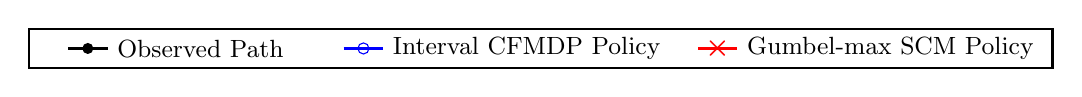
\begin{tikzpicture}[scale=1.0, every node/.style={scale=1.0}]
            \draw[thick, black] (-3, -0.25) rectangle (10, 0.25);
            %
            \draw[black, line width=1pt] (-2.5, 0.0) -- (-2,0.0);
            \fill[black] (-2.25,0.0) circle (2pt); %
            \node[right] at (-2,0.0) {\small Observed Path};
            
            %
            \draw[blue, line width=1pt] (1.0,0.0) -- (1.5,0.0);
            \node[draw=blue, circle, minimum size=4pt, inner sep=0pt] at (1.25,0.0) {}; %
            \node[right] at (1.5,0.0) {\small Interval CFMDP Policy};
            
            %
            \draw[red, line width=1pt] (5.5,0) -- (6,0);
            \node[red] at (5.75,0) {$\boldsymbol{\times}$}; %
            \node[right] at (6,0) {\small Gumbel-max SCM Policy};
        \end{tikzpicture}
    }\\
    %
    \subfigure[\footnotesize Lowest cumulative reward: Interval CFMDP ($312$), Gumbel-max SCM ($312$)]{%
        \resizebox{0.76\columnwidth}{!}{
             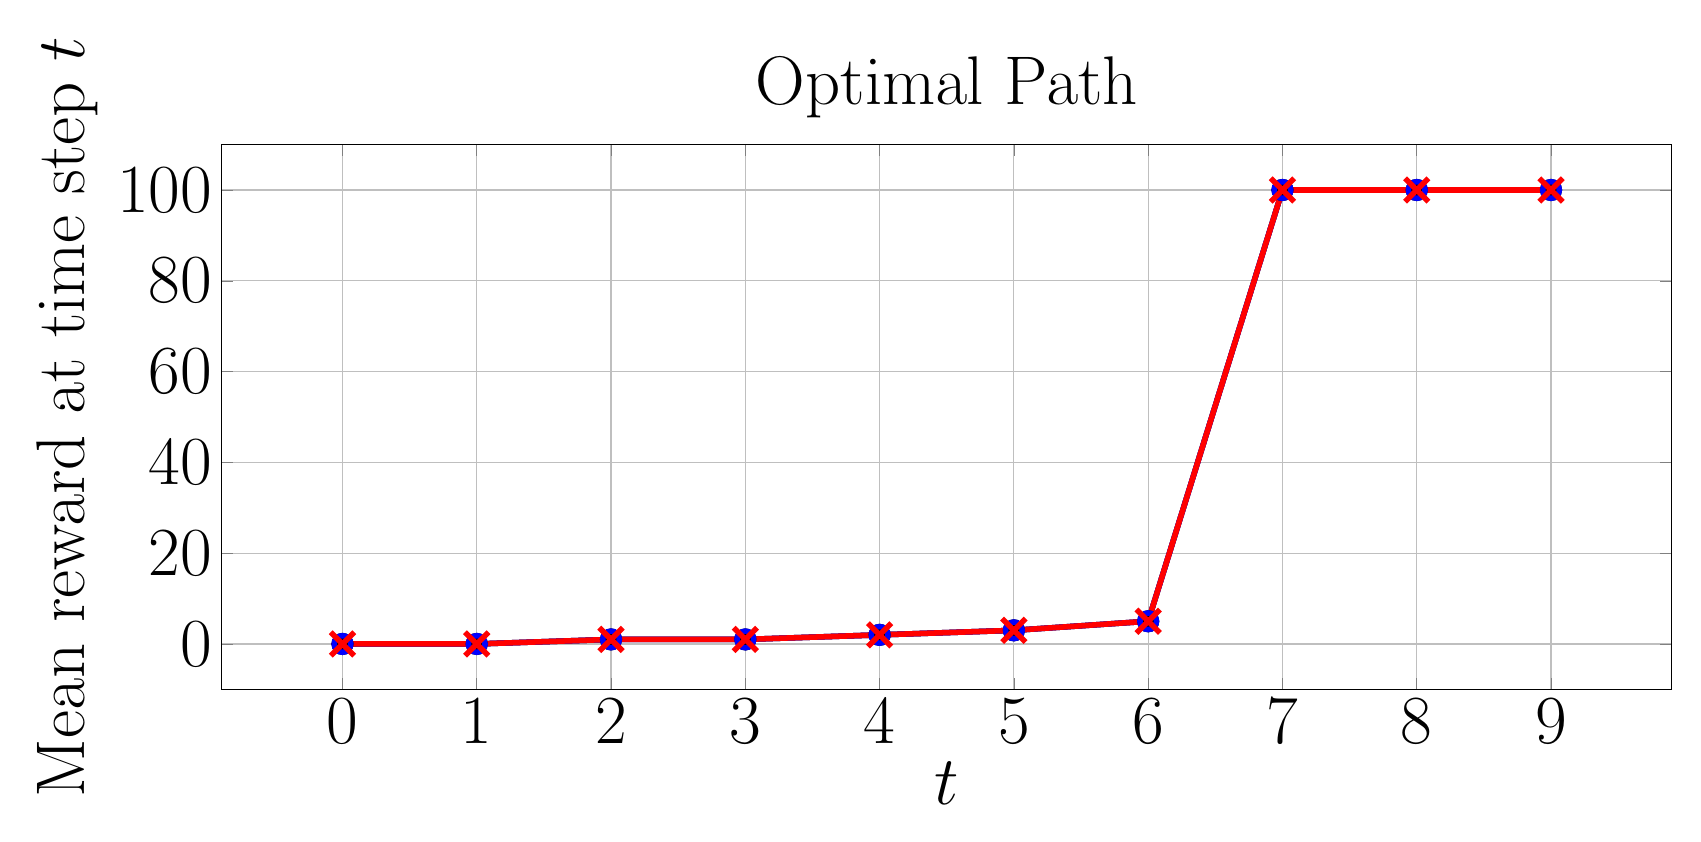
\begin{tikzpicture}
                \begin{axis}[
                    xlabel={$t$},
                    ylabel={Mean reward at time step $t$},
                    title={Optimal Path},
                    grid=both,
                    width=20cm, height=8.5cm,
                    every axis/.style={font=\Huge},
                    %
                ]
                \addplot[
                    color=black, %
                    mark=*, %
                    line width=2pt,
                    mark size=3pt,
                    error bars/.cd,
                    y dir=both, %
                    y explicit, %
                    error bar style={line width=1pt,solid},
                    error mark options={line width=1pt,mark size=4pt,rotate=90}
                ]
                coordinates {
                    (0, 0.0)  +- (0, 0.0)
                    (1, 0.0)  +- (0, 0.0) 
                    (2, 1.0)  +- (0, 0.0) 
                    (3, 1.0)  +- (0, 0.0)
                    (4, 2.0)  +- (0, 0.0)
                    (5, 3.0) +- (0, 0.0)
                    (6, 5.0) +- (0, 0.0)
                    (7, 100.0) +- (0, 0.0)
                    (8, 100.0) +- (0, 0.0)
                    (9, 100.0) +- (0, 0.0)
                };
                %
                \addplot[
                    color=blue, %
                    mark=o, %
                    line width=2pt,
                    mark size=3pt,
                    error bars/.cd,
                    y dir=both, %
                    y explicit, %
                    error bar style={line width=1pt,solid},
                    error mark options={line width=1pt,mark size=4pt,rotate=90}
                ]
                 coordinates {
                    (0, 0.0)  +- (0, 0.0)
                    (1, 0.0)  +- (0, 0.0) 
                    (2, 1.0)  +- (0, 0.0) 
                    (3, 1.0)  +- (0, 0.0)
                    (4, 2.0)  +- (0, 0.0)
                    (5, 3.0) +- (0, 0.0)
                    (6, 5.0) +- (0, 0.0)
                    (7, 100.0) +- (0, 0.0)
                    (8, 100.0) +- (0, 0.0)
                    (9, 100.0) +- (0, 0.0)
                };
                %
                \addplot[
                    color=red, %
                    mark=x, %
                    line width=2pt,
                    mark size=6pt,
                    error bars/.cd,
                    y dir=both, %
                    y explicit, %
                    error bar style={line width=1pt,solid},
                    error mark options={line width=1pt,mark size=4pt,rotate=90}
                ]
                coordinates {
                    (0, 0.0)  +- (0, 0.0)
                    (1, 0.0)  +- (0, 0.0) 
                    (2, 1.0)  +- (0, 0.0) 
                    (3, 1.0)  +- (0, 0.0)
                    (4, 2.0)  +- (0, 0.0)
                    (5, 3.0) +- (0, 0.0)
                    (6, 5.0) +- (0, 0.0)
                    (7, 100.0) +- (0, 0.0)
                    (8, 100.0) +- (0, 0.0)
                    (9, 100.0) +- (0, 0.0)
                };
                \end{axis}
            \end{tikzpicture}
         }
    }
    \hspace{1cm}
    \subfigure[\footnotesize Lowest cumulative reward: Interval CFMDP ($19$), Gumbel-max SCM ($-88$)]{%
         \resizebox{0.76\columnwidth}{!}{
            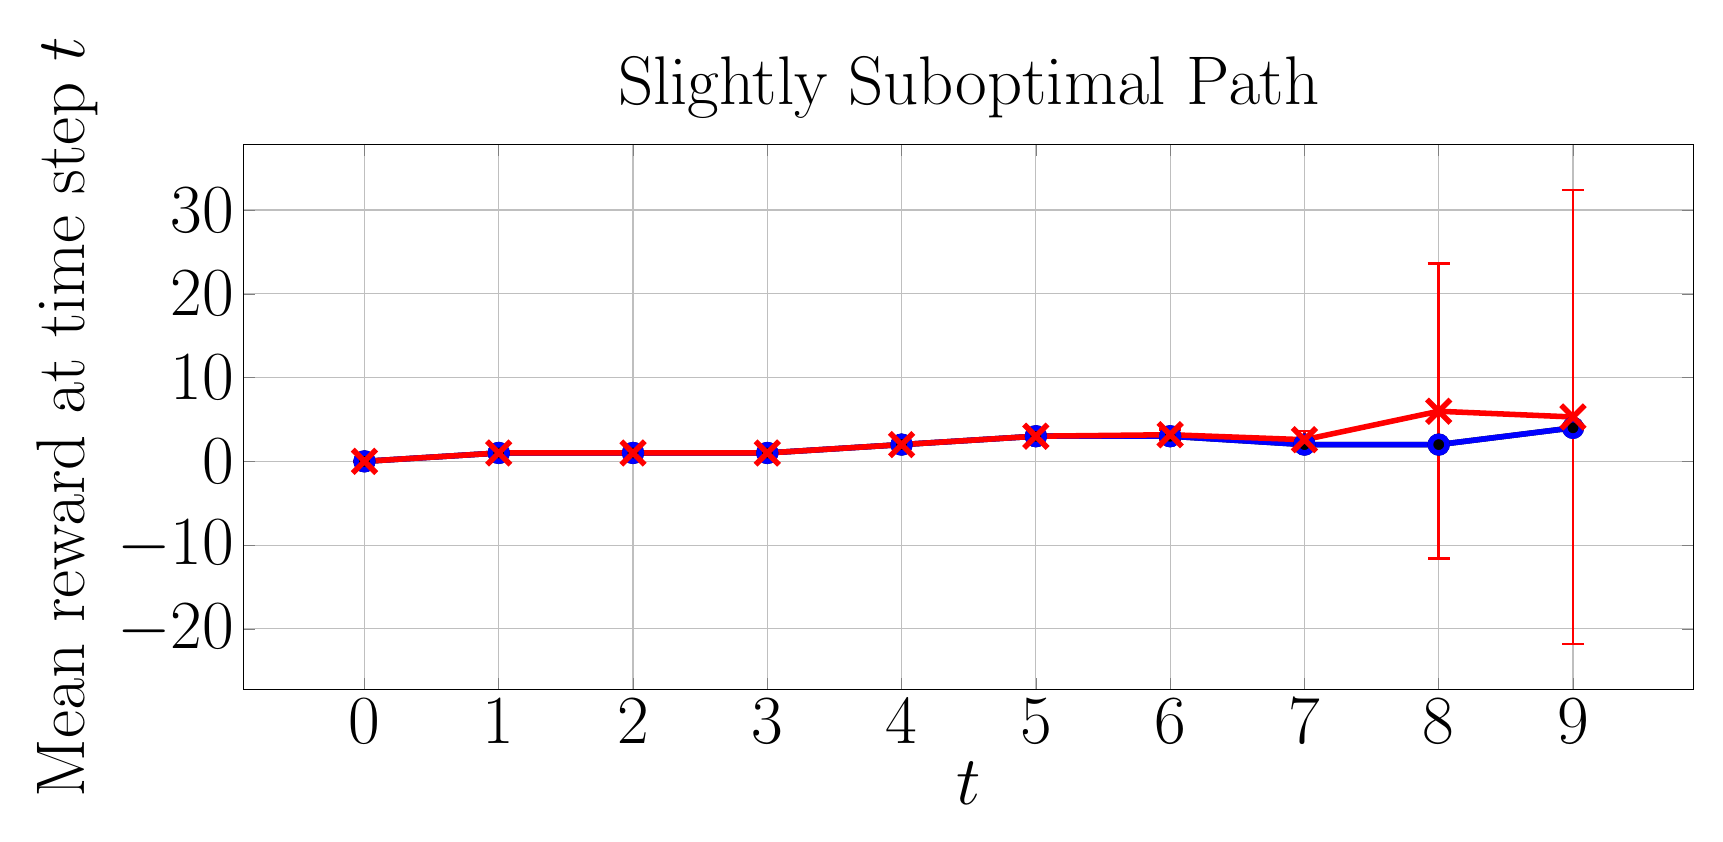
\begin{tikzpicture}
                \begin{axis}[
                    xlabel={$t$},
                    ylabel={Mean reward at time step $t$},
                    title={Slightly Suboptimal Path},
                    grid=both,
                    width=20cm, height=8.5cm,
                    every axis/.style={font=\Huge},
                    %
                ]
                \addplot[
                    color=black, %
                    mark=*, %
                    line width=2pt,
                    mark size=3pt,
                    error bars/.cd,
                    y dir=both, %
                    y explicit, %
                    error bar style={line width=1pt,solid},
                    error mark options={line width=1pt,mark size=4pt,rotate=90}
                ]
              coordinates {
                    (0, 0.0)  +- (0, 0.0)
                    (1, 1.0)  +- (0, 0.0) 
                    (2, 1.0)  +- (0, 0.0) 
                    (3, 1.0)  +- (0, 0.0)
                    (4, 2.0)  +- (0, 0.0)
                    (5, 3.0) +- (0, 0.0)
                    (6, 3.0) +- (0, 0.0)
                    (7, 2.0) +- (0, 0.0)
                    (8, 2.0) +- (0, 0.0)
                    (9, 4.0) +- (0, 0.0)
                };
                %
                \addplot[
                    color=blue, %
                    mark=o, %
                    line width=2pt,
                    mark size=3pt,
                    error bars/.cd,
                    y dir=both, %
                    y explicit, %
                    error bar style={line width=1pt,solid},
                    error mark options={line width=1pt,mark size=4pt,rotate=90}
                ]
              coordinates {
                    (0, 0.0)  +- (0, 0.0)
                    (1, 1.0)  +- (0, 0.0) 
                    (2, 1.0)  +- (0, 0.0) 
                    (3, 1.0)  +- (0, 0.0)
                    (4, 2.0)  +- (0, 0.0)
                    (5, 3.0) +- (0, 0.0)
                    (6, 3.0) +- (0, 0.0)
                    (7, 2.0) +- (0, 0.0)
                    (8, 2.0) +- (0, 0.0)
                    (9, 4.0) +- (0, 0.0)
                };
                %
                \addplot[
                    color=red, %
                    mark=x, %
                    line width=2pt,
                    mark size=6pt,
                    error bars/.cd,
                    y dir=both, %
                    y explicit, %
                    error bar style={line width=1pt,solid},
                    error mark options={line width=1pt,mark size=4pt,rotate=90}
                ]
                coordinates {
                    (0, 0.0)  +- (0, 0.0)
                    (1, 1.0)  +- (0, 0.0) 
                    (2, 1.0)  +- (0, 0.0) 
                    (3, 1.0)  +- (0, 0.0)
                    (4, 2.0)  += (0, 0.0)
                    (5, 3.0)  += (0, 0.0)
                    (6, 3.17847) += (0, 0.62606746) -= (0, 0.62606746)
                    (7, 2.5832885) += (0, 1.04598233) -= (0, 1.04598233)
                    (8, 5.978909) += (0, 17.60137623) -= (0, 17.60137623)
                    (9, 5.297059) += (0, 27.09227512) -= (0, 27.09227512)
                };
                \end{axis}
            \end{tikzpicture}
         }
    }\\[-1.5pt]
    \subfigure[\footnotesize Lowest cumulative reward: Interval CFMDP ($14$), Gumbel-max SCM ($-598$)]{%
         \resizebox{0.76\columnwidth}{!}{
             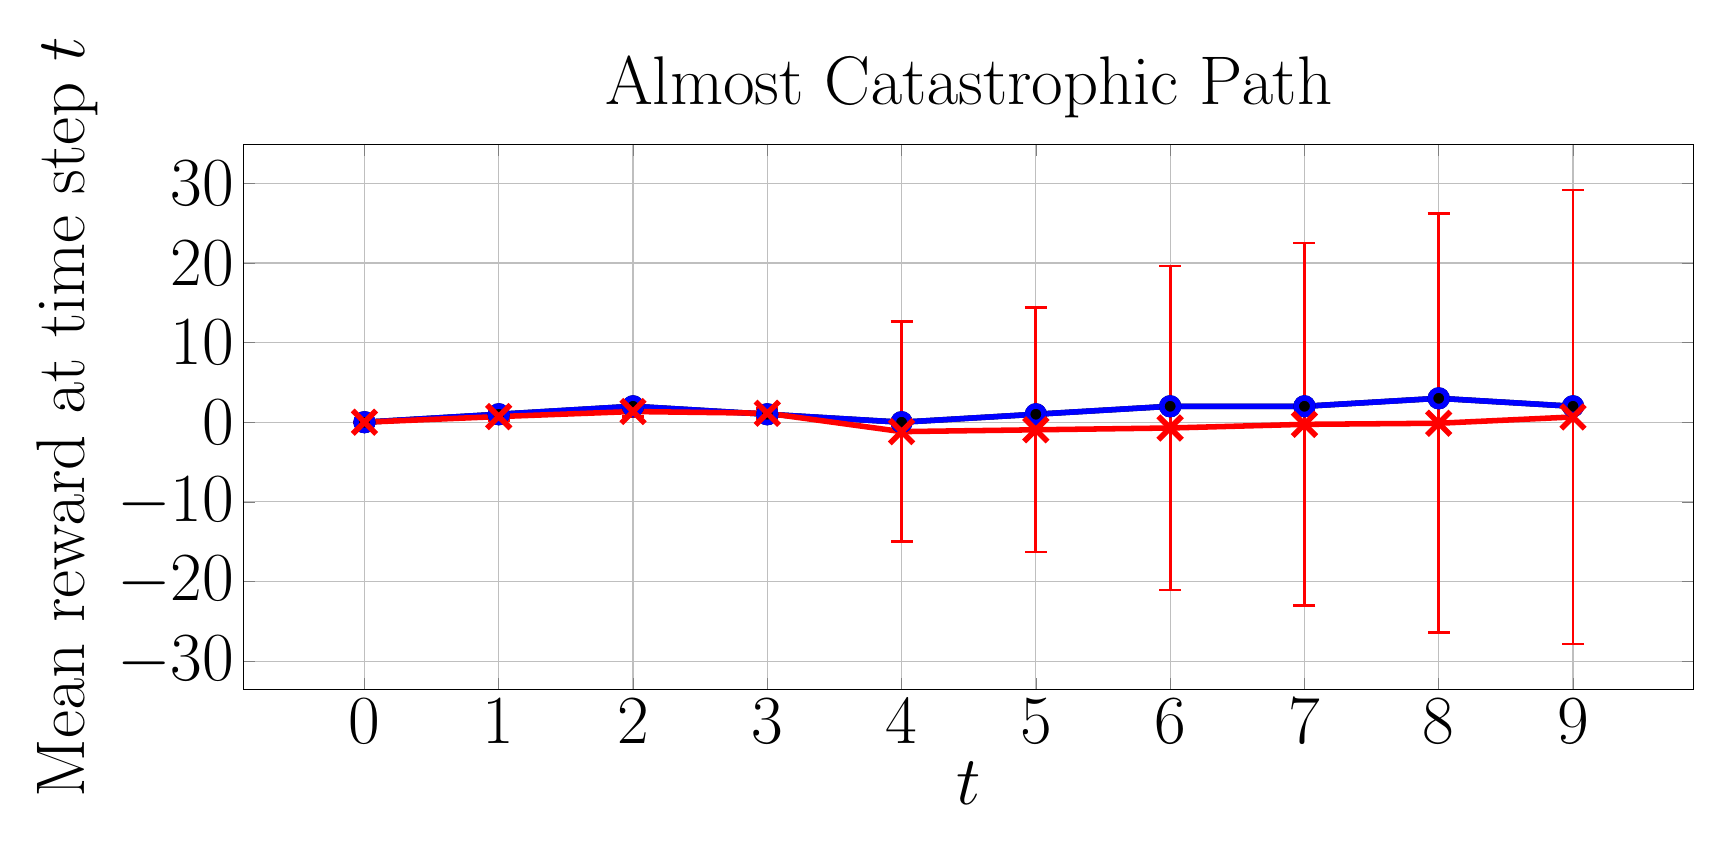
\begin{tikzpicture}
                \begin{axis}[
                    xlabel={$t$},
                    ylabel={Mean reward at time step $t$},
                    title={Almost Catastrophic Path},
                    grid=both,
                    width=20cm, height=8.5cm,
                    every axis/.style={font=\Huge},
                    %
                ]
                \addplot[
                    color=black, %
                    mark=*, %
                    line width=2pt,
                    mark size=3pt,
                    error bars/.cd,
                    y dir=both, %
                    y explicit, %
                    error bar style={line width=1pt,solid},
                    error mark options={line width=1pt,mark size=4pt,rotate=90}
                ]
                coordinates {
                    (0, 0.0)  +- (0, 0.0)
                    (1, 1.0)  +- (0, 0.0) 
                    (2, 2.0)  +- (0, 0.0) 
                    (3, 1.0)  +- (0, 0.0)
                    (4, 0.0)  +- (0, 0.0)
                    (5, 1.0) +- (0, 0.0)
                    (6, 2.0) +- (0, 0.0)
                    (7, 2.0) +- (0, 0.0)
                    (8, 3.0) +- (0, 0.0)
                    (9, 2.0) +- (0, 0.0)
                };
                %
                \addplot[
                    color=blue, %
                    mark=o, %
                    line width=2pt,
                    mark size=3pt,
                    error bars/.cd,
                    y dir=both, %
                    y explicit, %
                    error bar style={line width=1pt,solid},
                    error mark options={line width=1pt,mark size=4pt,rotate=90}
                ]
                coordinates {
                    (0, 0.0)  +- (0, 0.0)
                    (1, 1.0)  +- (0, 0.0) 
                    (2, 2.0)  +- (0, 0.0) 
                    (3, 1.0)  +- (0, 0.0)
                    (4, 0.0)  +- (0, 0.0)
                    (5, 1.0) +- (0, 0.0)
                    (6, 2.0) +- (0, 0.0)
                    (7, 2.0) +- (0, 0.0)
                    (8, 3.0) +- (0, 0.0)
                    (9, 2.0) +- (0, 0.0)
                };
                %
                \addplot[
                    color=red, %
                    mark=x, %
                    line width=2pt,
                    mark size=6pt,
                    error bars/.cd,
                    y dir=both, %
                    y explicit, %
                    error bar style={line width=1pt,solid},
                    error mark options={line width=1pt,mark size=4pt,rotate=90}
                ]
                coordinates {
                    (0, 0.0)  +- (0, 0.0)
                    (1, 0.7065655)  +- (0, 0.4553358) 
                    (2, 1.341673)  +- (0, 0.67091621) 
                    (3, 1.122926)  +- (0, 0.61281824)
                    (4, -1.1821935)  +- (0, 13.82444042)
                    (5, -0.952399)  +- (0, 15.35195457)
                    (6, -0.72672) +- (0, 20.33508414)
                    (7, -0.268983) +- (0, 22.77861454)
                    (8, -0.1310835) +- (0, 26.31013314)
                    (9, 0.65806) +- (0, 28.50670214)
                };
                %
            %
            %
            %
            %
            %
            %
            %
            %
            %
            %
            %
            %
            %
            %
            %
            %
            %
            %
                \end{axis}
            \end{tikzpicture}
         }
    }
    \hspace{1cm}
    \subfigure[\footnotesize Lowest cumulative reward: Interval CFMDP ($-698$), Gumbel-max SCM ($-698$)]{%
         \resizebox{0.76\columnwidth}{!}{
            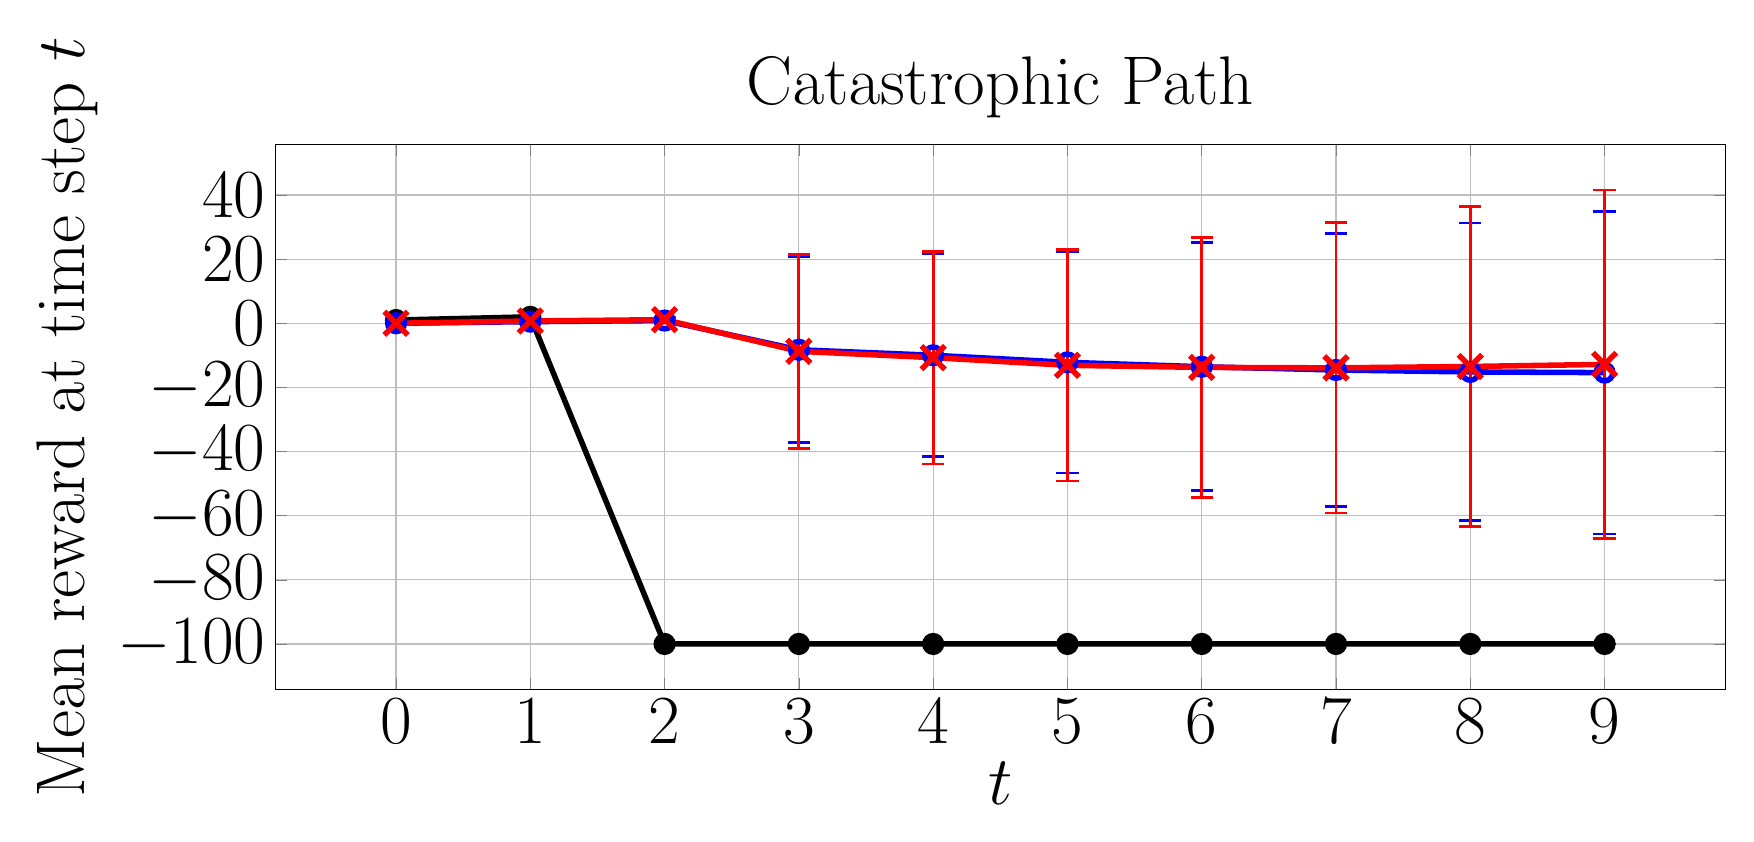
\begin{tikzpicture}
                \begin{axis}[
                    xlabel={$t$},
                    ylabel={Mean reward at time step $t$},
                    title={Catastrophic Path},
                    grid=both,
                    width=20cm, height=8.5cm,
                    every axis/.style={font=\Huge},
                    %
                ]
                \addplot[
                    color=black, %
                    mark=*, %
                    line width=2pt,
                    mark size=3pt,
                    error bars/.cd,
                    y dir=both, %
                    y explicit, %
                    error bar style={line width=1pt,solid},
                    error mark options={line width=1pt,mark size=4pt,rotate=90}
                ]
                coordinates {
                    (0, 1.0)  +- (0, 0.0)
                    (1, 2.0)  +- (0, 0.0) 
                    (2, -100.0)  +- (0, 0.0) 
                    (3, -100.0)  +- (0, 0.0)
                    (4, -100.0)  +- (0, 0.0)
                    (5, -100.0) +- (0, 0.0)
                    (6, -100.0) +- (0, 0.0)
                    (7, -100.0) +- (0, 0.0)
                    (8, -100.0) +- (0, 0.0)
                    (9, -100.0) +- (0, 0.0)
                };
                %
                \addplot[
                    color=blue, %
                    mark=o, %
                    line width=2pt,
                    mark size=3pt,
                    error bars/.cd,
                    y dir=both, %
                    y explicit, %
                    error bar style={line width=1pt,solid},
                    error mark options={line width=1pt,mark size=4pt,rotate=90}
                ]
                coordinates {
                    (0, 0.0)  +- (0, 0.0)
                    (1, 0.504814)  +- (0, 0.49997682) 
                    (2, 0.8439835)  +- (0, 0.76831917) 
                    (3, -8.2709165)  +- (0, 28.93656754)
                    (4, -9.981082)  +- (0, 31.66825363)
                    (5, -12.1776325) +- (0, 34.53463233)
                    (6, -13.556076) +- (0, 38.62845372)
                    (7, -14.574418) +- (0, 42.49603359)
                    (8, -15.1757075) +- (0, 46.41913968)
                    (9, -15.3900395) +- (0, 50.33563368)
                };
                %
                \addplot[
                    color=red, %
                    mark=x, %
                    line width=2pt,
                    mark size=6pt,
                    error bars/.cd,
                    y dir=both, %
                    y explicit, %
                    error bar style={line width=1pt,solid},
                    error mark options={line width=1pt,mark size=4pt,rotate=90}
                ]
                coordinates {
                    (0, 0.0)  +- (0, 0.0)
                    (1, 0.701873)  +- (0, 0.45743556) 
                    (2, 1.1227805)  +- (0, 0.73433129) 
                    (3, -8.7503255)  +- (0, 30.30257976)
                    (4, -10.722092)  +- (0, 33.17618589)
                    (5, -13.10721)  +- (0, 36.0648089)
                    (6, -13.7631645) +- (0, 40.56553451)
                    (7, -13.909043) +- (0, 45.23829402)
                    (8, -13.472517) +- (0, 49.96270296)
                    (9, -12.8278835) +- (0, 54.38618735)
                };
                %
            %
            %
            %
            %
            %
            %
            %
            %
            %
            %
            %
            %
            %
            %
            %
            %
            %
            %
                \end{axis}
            \end{tikzpicture}
         }
    }
    \caption{Average instant reward of CF paths induced by policies on GridWorld $p=0.4$.}
    \label{fig: reward p=0.4}
\end{figure*}

\subsection{Experimental Setup}
To compare policy performance, we measure the average rewards of counterfactual paths induced by our policy and the Gumbel-max policy by uniformly sampling $200$ counterfactual MDPs from the ICFMDP and generating $10,000$ counterfactual paths over each sampled CFMDP. \jl{Since the interval CFMDP depends on the observed path, we select $4$  paths of varying optimality to evaluate how the observed path impacts the performance of both policies: an optimal path, a slightly suboptimal path that could reach the optimal reward with a few changes, a catastrophic path that enters a catastrophic, terminal state with low reward, and an almost catastrophic path that was close to entering a catastrophic state.} When measuring the average probability bound widths and execution time needed to generate the ICFMDPs, we averaged over $20$ randomly generated observed paths
\footnote{Further training details are provided in Appendix \ref{app: training details}, and the code is provided at \href{https://github.com/ddv-lab/robust-cf-inference-in-MDPs}{https://github.com/ddv-lab/robust-cf-inference-in-MDPs}
%
%
.}.

\subsection{GridWorld}
\jl{The GridWorld MDP is a $4 \times 4$ grid where an agent must navigate from the top-left corner to the goal state in the bottom-right corner, avoiding a dangerous terminal state in the centre. At each time step, the agent can move up, down, left, or right, but there is a small probability (controlled by hyper-parameter $p$) of moving in an unintended direction. As the agent nears the goal, the reward for each state increases, culminating in a reward of $+100$ for reaching the goal. Entering the dangerous state results in a penalty of $-100$. We use two versions of GridWorld: a less stochastic version with $p=0.9$ (i.e., $90$\% chance of moving in the chosen direction) and a more stochastic version with $p=0.4$.}

\paragraph{GridWorld ($p=0.9$)}
When $p=0.9$, the counterfactual probability bounds are typically narrow (see Table \ref{tab:nonzero_probs} for average measurements). Consequently, as shown in Figure \ref{fig: reward p=0.9}, both policies are nearly identical and perform similarly well across the optimal, slightly suboptimal, and catastrophic paths.
%
However, for the almost catastrophic path, the interval CFMDP path is more conservative and follows the observed path more closely (as this is where the probability bounds are narrowest), which typically requires one additional step to reach the goal state than the Gumbel-max SCM policy.
%

\paragraph{GridWorld ($p=0.4$)}
\jl{When $p=0.4$, the GridWorld environment becomes more uncertain, increasing the risk of entering the dangerous state even if correct actions are chosen. Thus, as shown in Figure \ref{fig: reward p=0.4}, the interval CFMDP policy adopts a more conservative approach, avoiding deviation from the observed policy if it cannot guarantee higher counterfactual rewards (see the slightly suboptimal and almost catastrophic paths), whereas the Gumbel-max SCM is inconsistent: it can yield higher rewards, but also much lower rewards, reflected in the wide error bars.} For the catastrophic path, both policies must deviate from the observed path to achieve a higher reward and, in this case, perform similarly.
%
%
%
%
\subsection{Sepsis}
The Sepsis MDP \citep{oberst2019counterfactual} simulates trajectories of Sepsis patients. Each state consists of four vital signs (heart rate, blood pressure, oxygen concentration, and glucose levels), categorised as low, normal, or high.
and three treatments that can be toggled on/off at each time step (8 actions in total). Unlike \citet{oberst2019counterfactual}, we scale rewards based on the number of out-of-range vital signs, between $-1000$ (patient dies) and $1000$ (patient discharged). \jl{Like the GridWorld $p=0.4$ experiment, the Sepsis MDP is highly uncertain, as many states are equally likely to lead to optimal and poor outcomes. Thus, as shown in Figure \ref{fig: reward sepsis}, both policies follow the observed optimal and almost catastrophic paths to guarantee rewards are no worse than the observation.} However, improving the catastrophic path requires deviating from the observation. Here, the Gumbel-max SCM policy, on average, performs better than the interval CFMDP policy. But, since both policies have lower bounds clipped at $-1000$, neither policy reliably improves over the observation. In contrast, for the slightly suboptimal path, the interval CFMDP policy performs significantly better, shown by its higher lower bounds. 
Moreover, in these two cases, the worst-case counterfactual path generated by the interval CFMDP policy is better than that of the Gumbel-max SCM policy,
indicating its greater robustness.
%
\begin{figure*}
    \centering
     \resizebox{0.6\textwidth}{!}{
        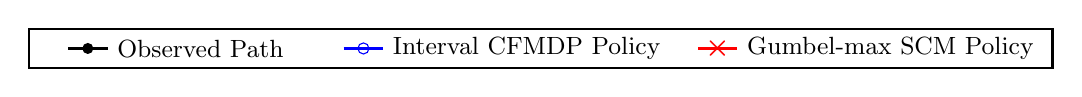
\begin{tikzpicture}[scale=1.0, every node/.style={scale=1.0}]
            \draw[thick, black] (-3, -0.25) rectangle (10, 0.25);
            %
            \draw[black, line width=1pt] (-2.5, 0.0) -- (-2,0.0);
            \fill[black] (-2.25,0.0) circle (2pt); %
            \node[right] at (-2,0.0) {\small Observed Path};
            
            %
            \draw[blue, line width=1pt] (1.0,0.0) -- (1.5,0.0);
            \node[draw=blue, circle, minimum size=4pt, inner sep=0pt] at (1.25,0.0) {}; %
            \node[right] at (1.5,0.0) {\small Interval CFMDP Policy};
            
            %
            \draw[red, line width=1pt] (5.5,0) -- (6,0);
            \node[red] at (5.75,0) {$\boldsymbol{\times}$}; %
            \node[right] at (6,0) {\small Gumbel-max SCM Policy};
        \end{tikzpicture}
    }\\
    \subfigure[\footnotesize Lowest cumulative reward: Interval CFMDP ($8000$), Gumbel-max SCM ($8000$)]{%
         \resizebox{0.76\columnwidth}{!}{
             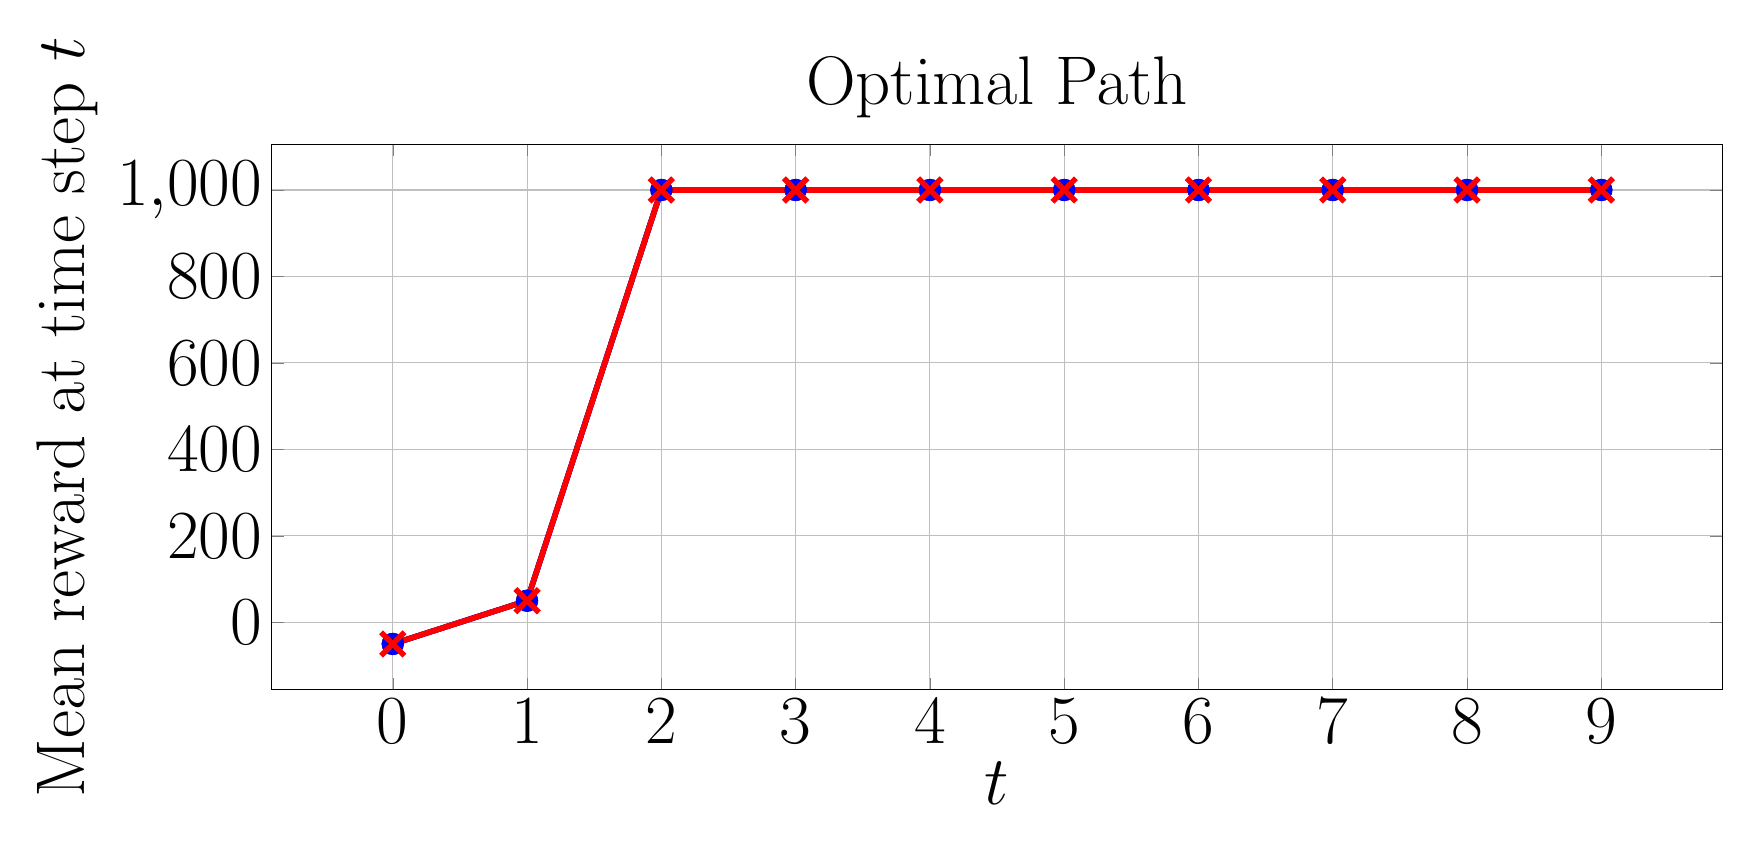
\begin{tikzpicture}
                \begin{axis}[
                    xlabel={$t$},
                    ylabel={Mean reward at time step $t$},
                    title={Optimal Path},
                    grid=both,
                    width=20cm, height=8.5cm,
                    every axis/.style={font=\Huge},
                    %
                ]
                \addplot[
                    color=black, %
                    mark=*, %
                    line width=2pt,
                    mark size=3pt,
                ]
                coordinates {
                    (0, -50.0)
                    (1, 50.0)
                    (2, 1000.0)
                    (3, 1000.0)
                    (4, 1000.0)
                    (5, 1000.0)
                    (6, 1000.0)
                    (7, 1000.0)
                    (8, 1000.0)
                    (9, 1000.0)
                };
                %
                \addplot[
                    color=blue, %
                    mark=o, %
                    line width=2pt,
                    mark size=3pt,
                    error bars/.cd,
                    y dir=both, %
                    y explicit, %
                    error bar style={line width=1pt,solid},
                    error mark options={line width=1pt,mark size=4pt,rotate=90}
                ]
                coordinates {
                    (0, -50.0)  +- (0, 0.0)
                    (1, 50.0)  +- (0, 0.0) 
                    (2, 1000.0)  +- (0, 0.0) 
                    (3, 1000.0)  +- (0, 0.0)
                    (4, 1000.0)  +- (0, 0.0)
                    (5, 1000.0) +- (0, 0.0)
                    (6, 1000.0) +- (0, 0.0)
                    (7, 1000.0) +- (0, 0.0)
                    (8, 1000.0) +- (0, 0.0)
                    (9, 1000.0) +- (0, 0.0)
                };
                %
                \addplot[
                    color=red, %
                    mark=x, %
                    line width=2pt,
                    mark size=6pt,
                    error bars/.cd,
                    y dir=both, %
                    y explicit, %
                    error bar style={line width=1pt,solid},
                    error mark options={line width=1pt,mark size=4pt,rotate=90}
                ]
                coordinates {
                    (0, -50.0)  +- (0, 0.0)
                    (1, 50.0)  +- (0, 0.0) 
                    (2, 1000.0)  +- (0, 0.0) 
                    (3, 1000.0)  +- (0, 0.0)
                    (4, 1000.0)  +- (0, 0.0)
                    (5, 1000.0) +- (0, 0.0)
                    (6, 1000.0) +- (0, 0.0)
                    (7, 1000.0) +- (0, 0.0)
                    (8, 1000.0) +- (0, 0.0)
                    (9, 1000.0) +- (0, 0.0)
                };
                %
                \end{axis}
            \end{tikzpicture}
         }
    }
    \hspace{1cm}
    \subfigure[\footnotesize Lowest cumulative reward: Interval CFMDP ($-5980$), Gumbel-max SCM ($-8000$)]{%
         \resizebox{0.76\columnwidth}{!}{
            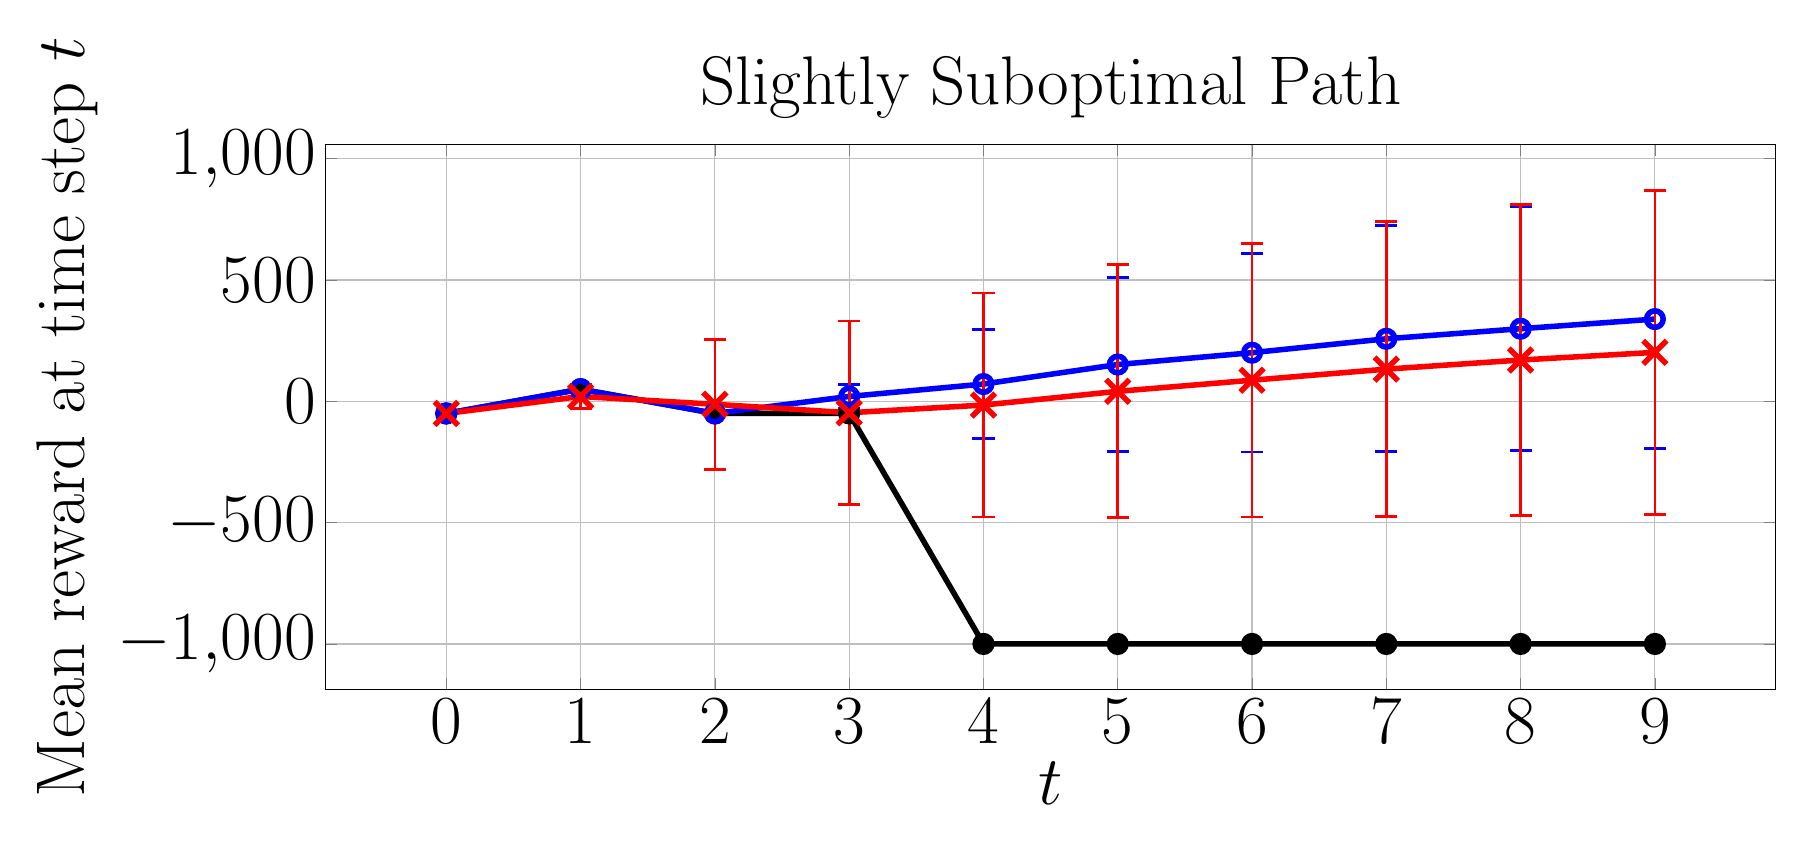
\begin{tikzpicture}
                \begin{axis}[
                    xlabel={$t$},
                    ylabel={Mean reward at time step $t$},
                    title={Slightly Suboptimal Path},
                    grid=both,
                    width=20cm, height=8.5cm,
                    every axis/.style={font=\Huge},
                    %
                ]
               \addplot[
                    color=black, %
                    mark=*, %
                    line width=2pt,
                    mark size=3pt,
                ]
                coordinates {
                    (0, -50.0)
                    (1, 50.0)
                    (2, -50.0)
                    (3, -50.0)
                    (4, -1000.0)
                    (5, -1000.0)
                    (6, -1000.0)
                    (7, -1000.0)
                    (8, -1000.0)
                    (9, -1000.0)
                };
                %
                \addplot[
                    color=blue, %
                    mark=o, %
                    line width=2pt,
                    mark size=3pt,
                    error bars/.cd,
                    y dir=both, %
                    y explicit, %
                    error bar style={line width=1pt,solid},
                    error mark options={line width=1pt,mark size=4pt,rotate=90}
                ]
                coordinates {
                    (0, -50.0)  +- (0, 0.0)
                    (1, 50.0)  +- (0, 0.0) 
                    (2, -50.0)  +- (0, 0.0) 
                    (3, 20.0631)  +- (0, 49.97539413)
                    (4, 71.206585)  +- (0, 226.02033693)
                    (5, 151.60797) +- (0, 359.23292559)
                    (6, 200.40593) +- (0, 408.86185176)
                    (7, 257.77948) +- (0, 466.10372804)
                    (8, 299.237465) +- (0, 501.82579506)
                    (9, 338.9129) +- (0, 532.06124996)
                };
                %
                \addplot[
                    color=red, %
                    mark=x, %
                    line width=2pt,
                    mark size=6pt,
                    error bars/.cd,
                    y dir=both, %
                    y explicit, %
                    error bar style={line width=1pt,solid},
                    error mark options={line width=1pt,mark size=4pt,rotate=90}
                ]
                coordinates {
                    (0, -50.0)  +- (0, 0.0)
                    (1, 20.00736)  +- (0, 49.99786741) 
                    (2, -12.282865)  +- (0, 267.598755) 
                    (3, -47.125995)  +- (0, 378.41755832)
                    (4, -15.381965)  +- (0, 461.77616558)
                    (5, 41.15459) +- (0, 521.53189262)
                    (6, 87.01595) +- (0, 564.22243126 )
                    (7, 132.62376) +- (0, 607.31338037)
                    (8, 170.168145) +- (0, 641.48013693)
                    (9, 201.813135) +- (0, 667.29441777)
                };
                %
                %
                %
                %
                %
                %
                %
                %
                %
                %
                %
                %
                %
                %
                %
                %
                %
                %
                %
                \end{axis}
            \end{tikzpicture}
         }
    }\\[-1.5pt]
    \subfigure[\footnotesize Lowest cumulative reward: Interval CFMDP ($100$), Gumbel-max SCM ($100$)]{%
         \resizebox{0.76\columnwidth}{!}{
             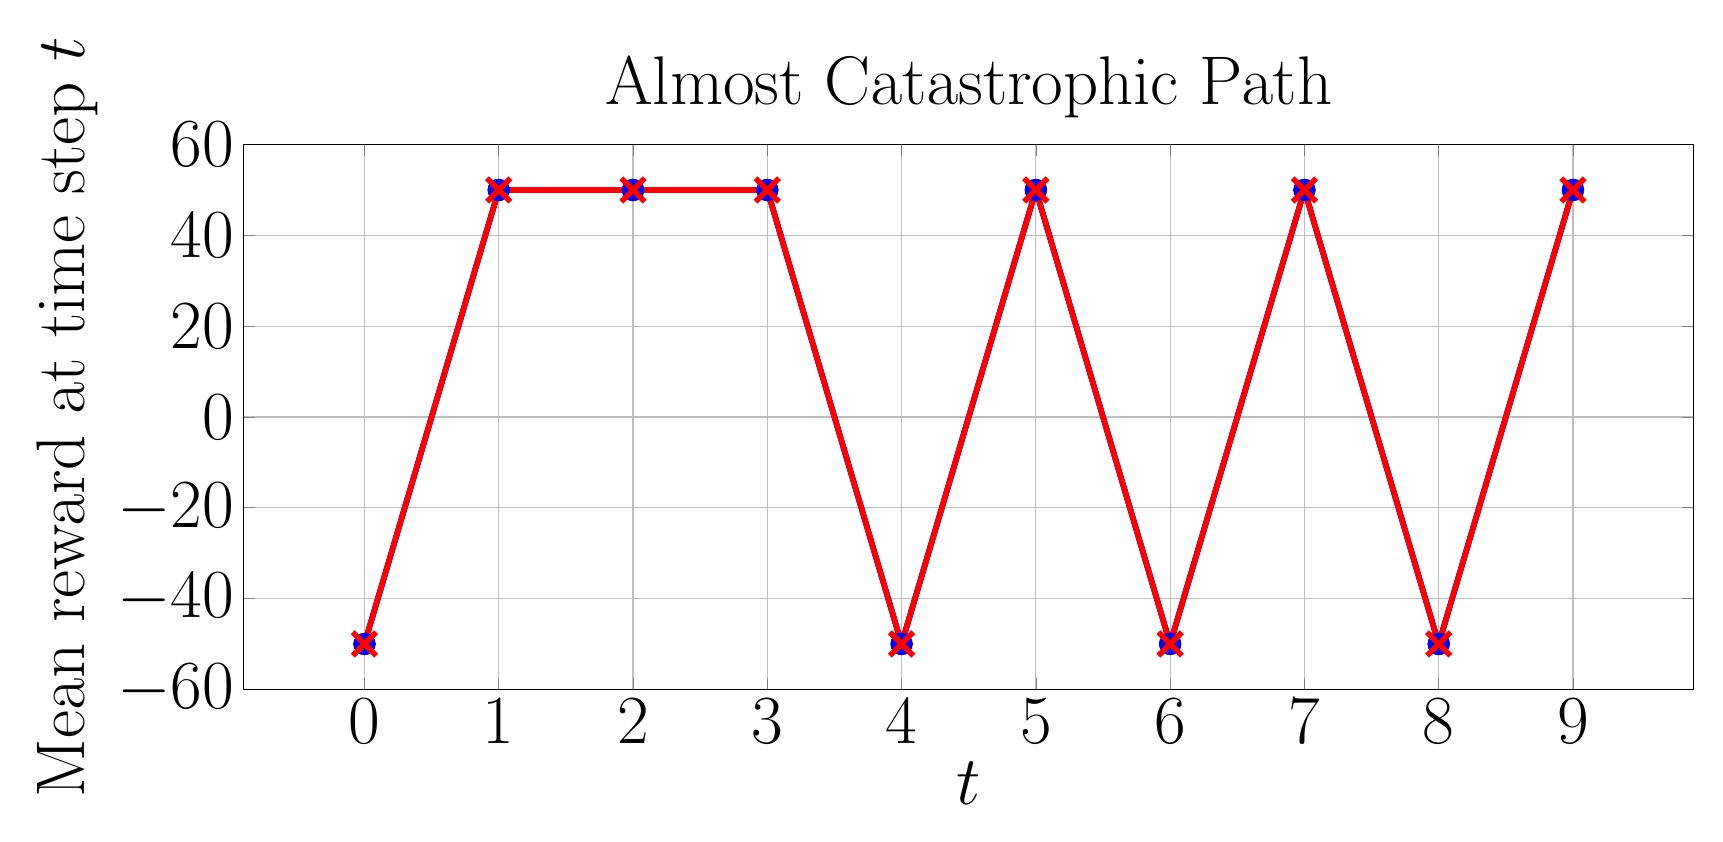
\begin{tikzpicture}
                \begin{axis}[
                    xlabel={$t$},
                    ylabel={Mean reward at time step $t$},
                    title={Almost Catastrophic Path},
                    grid=both,
                    every axis/.style={font=\Huge},
                    width=20cm, height=8.5cm,
                    %
                ]
               \addplot[
                    color=black, %
                    mark=*, %
                    line width=2pt,
                    mark size=3pt,
                ]
                coordinates {
                    (0, -50.0)
                    (1, 50.0)
                    (2, 50.0)
                    (3, 50.0)
                    (4, -50.0)
                    (5, 50.0)
                    (6, -50.0)
                    (7, 50.0)
                    (8, -50.0)
                    (9, 50.0)
                };
                %
                %
                \addplot[
                    color=blue, %
                    mark=o, %
                    line width=2pt,
                    mark size=3pt,
                    error bars/.cd,
                    y dir=both, %
                    y explicit, %
                    error bar style={line width=1pt,solid},
                    error mark options={line width=1pt,mark size=4pt,rotate=90}
                ]
                coordinates {
                    (0, -50.0)  +- (0, 0.0)
                    (1, 50.0)  +- (0, 0.0) 
                    (2, 50.0)  +- (0, 0.0) 
                    (3, 50.0)  +- (0, 0.0)
                    (4, -50.0)  +- (0, 0.0)
                    (5, 50.0) +- (0, 0.0)
                    (6, -50.0) +- (0, 0.0)
                    (7, 50.0) +- (0, 0.0)
                    (8, -50.0) +- (0, 0.0)
                    (9, 50.0) +- (0, 0.0)
                };
                %
                \addplot[
                    color=red, %
                    mark=x, %
                    line width=2pt,
                    mark size=6pt,
                    error bars/.cd,
                    y dir=both, %
                    y explicit, %
                    error bar style={line width=1pt,solid},
                    error mark options={line width=1pt,mark size=4pt,rotate=90}
                ]
                coordinates {
                    (0, -50.0)  +- (0, 0.0)
                    (1, 50.0)  +- (0, 0.0) 
                    (2, 50.0)  +- (0, 0.0) 
                    (3, 50.0)  +- (0, 0.0)
                    (4, -50.0)  +- (0, 0.0)
                    (5, 50.0) +- (0, 0.0)
                    (6, -50.0) +- (0, 0.0)
                    (7, 50.0) +- (0, 0.0)
                    (8, -50.0) +- (0, 0.0)
                    (9, 50.0) +- (0, 0.0)
                };
                %
                %
                %
                %
                %
                %
                %
                %
                %
                %
                %
                %
                %
                %
                %
                %
                %
                %
                %
                \end{axis}
            \end{tikzpicture}
         }
    }
    \hspace{1cm}
    \subfigure[\footnotesize Lowest cumulative reward: Interval CFMDP ($-7150$), Gumbel-max SCM ($-9050$)]{%
         \resizebox{0.76\columnwidth}{!}{
            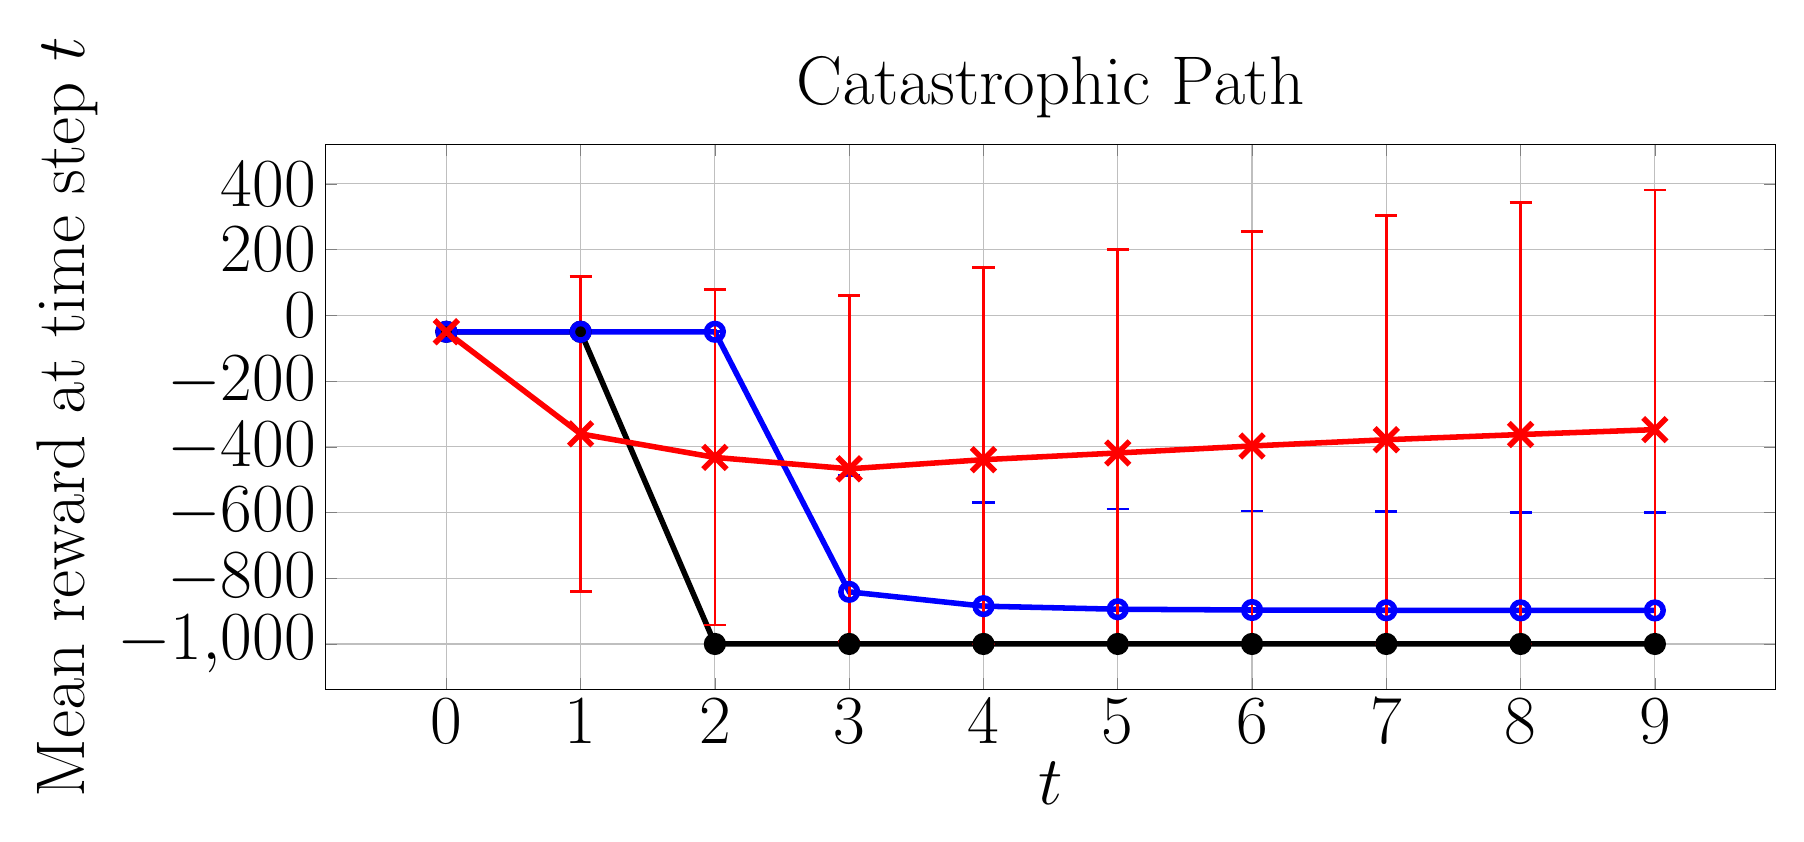
\begin{tikzpicture}
                \begin{axis}[
                    xlabel={$t$},
                    ylabel={Mean reward at time step $t$},
                    title={Catastrophic Path},
                    grid=both,
                    width=20cm, height=8.5cm,
                    every axis/.style={font=\Huge},
                    %
                ]
               \addplot[
                    color=black, %
                    mark=*, %
                    line width=2pt,
                    mark size=3pt,
                ]
                coordinates {
                    (0, -50.0)
                    (1, -50.0)
                    (2, -1000.0)
                    (3, -1000.0)
                    (4, -1000.0)
                    (5, -1000.0)
                    (6, -1000.0)
                    (7, -1000.0)
                    (8, -1000.0)
                    (9, -1000.0)
                };
                %
                %
                \addplot[
                    color=blue, %
                    mark=o, %
                    line width=2pt,
                    mark size=3pt,
                    error bars/.cd,
                    y dir=both, %
                    y explicit, %
                    error bar style={line width=1pt,solid},
                    error mark options={line width=1pt,mark size=4pt,rotate=90}
                ]
                coordinates {
                    (0, -50.0)  +- (0, 0.0)
                    (1, -50.0)  +- (0, 0.0) 
                    (2, -50.0)  +- (0, 0.0) 
                    (3, -841.440725)  += (0, 354.24605512) -= (0, 158.559275)
                    (4, -884.98225)  += (0, 315.37519669) -= (0, 115.01775)
                    (5, -894.330425) += (0, 304.88572805) -= (0, 105.669575)
                    (6, -896.696175) += (0, 301.19954514) -= (0, 103.303825)
                    (7, -897.4635) += (0, 299.61791279) -= (0, 102.5365)
                    (8, -897.77595) += (0, 298.80392585) -= (0, 102.22405)
                    (9, -897.942975) += (0, 298.32920557) -= (0, 102.057025)
                };
                %
                \addplot[
                    color=red, %
                    mark=x, %
                    line width=2pt,
                    mark size=6pt,
                    error bars/.cd,
                    y dir=both, %
                    y explicit, %
                    error bar style={line width=1pt,solid},
                    error mark options={line width=1pt,mark size=4pt,rotate=90}
                ]
            coordinates {
                    (0, -50.0)  +- (0, 0.0)
                    (1, -360.675265)  +- (0, 479.39812699) 
                    (2, -432.27629)  +- (0, 510.38620897) 
                    (3, -467.029545)  += (0, 526.36009628) -= (0, 526.36009628)
                    (4, -439.17429)  += (0, 583.96638919) -= (0, 560.82571)
                    (5, -418.82704) += (0, 618.43027478) -= (0, 581.17296)
                    (6, -397.464895) += (0, 652.67322574) -= (0, 602.535105)
                    (7, -378.49052) += (0, 682.85407033) -= (0, 621.50948)
                    (8, -362.654195) += (0, 707.01412023) -= (0, 637.345805)
                    (9, -347.737935) += (0, 729.29076479) -= (0, 652.262065)
                };
                %
                %
                %
                %
                %
                %
                %
                %
                %
                %
                %
                %
                %
                %
                %
                %
                %
                %
                %
                \end{axis}
            \end{tikzpicture}
         }
    }
    \caption{Average instant reward of CF paths induced by policies on Sepsis.}
    \label{fig: reward sepsis}
\end{figure*}

%
%
%
\subsection{Interval CFMDP Bounds}
%
%
Table \ref{tab:nonzero_probs} presents the mean counterfactual probability bound widths (excluding transitions where the upper bound is $0$) for each MDP, averaged over 20 observed paths. We compare the bounds under counterfactual stability (CS) and monotonicity (M) assumptions, CS alone, and no assumptions. This shows that the assumptions marginally reduce the bound widths, indicating the assumptions tighten the bounds without excluding too many causal models, as intended.
\renewcommand{\arraystretch}{1}

\begin{table}
\centering
\caption{Mean width of counterfactual probability bounds}
\resizebox{0.8\columnwidth}{!}{%
\begin{tabular}{|c|c|c|c|}
\hline
\multirow{2}{*}{\textbf{Environment}} & \multicolumn{3}{c|}{\textbf{Assumptions}} \\ \cline{2-4}
 & \textbf{CS + M} & \textbf{CS} & \textbf{None\tablefootnote{\jl{Equivalent to \citet{li2024probabilities}'s bounds (see Section \ref{sec: equivalence with Li}).}}} \\ \hline
\textbf{GridWorld} ($p=0.9$) & 0.0817 & 0.0977 & 0.100 \\ \hline
\textbf{GridWorld} ($p=0.4$) & 0.552  & 0.638  & 0.646 \\ \hline
\textbf{Sepsis} & 0.138 & 0.140 & 0.140 \\ \hline
\end{tabular}
}
\label{tab:nonzero_probs}
\end{table}


\subsection{Execution Times}
Table \ref{tab: times} compares the average time needed to generate the interval CFMDP vs.\ the Gumbel-max SCM CFMDP for 20 observations.
The GridWorld algorithms were run single-threaded, while the Sepsis experiments were run in parallel.
Generating the interval CFMDP is significantly faster as it uses exact analytical bounds, whereas the Gumbel-max CFMDP requires sampling from the Gumbel distribution to estimate counterfactual transition probabilities. \jl{Since constructing the counterfactual MDP models is the main bottleneck in both approaches, ours is more efficient overall and suitable for larger MDPs.}
\begin{table}
\centering
\caption{Mean execution time to generate CFMDPs}
\resizebox{0.99\columnwidth}{!}{%
\begin{tabular}{|c|c|c|}
\hline
\multirow{2}{*}{\textbf{Environment}} & \multicolumn{2}{c|}{\textbf{Mean Execution Time (s)}} \\ \cline{2-3} 
                                      & \textbf{Interval CFMDP} & \textbf{Gumbel-max CFMDP} \\ \hline
\textbf{GridWorld ($p=0.9$) }                  & 0.261                   & 56.1                      \\ \hline
\textbf{GridWorld ($p=0.4$)  }                 & 0.336                   & 54.5                      \\ \hline
\textbf{Sepsis}                                 & 688                     & 2940                      \\ \hline
\end{tabular}%
}
\label{tab: times}
\end{table}

\section{Conclusion}
In this work, we propose a simple yet effective approach, called SMILE, for graph few-shot learning with fewer tasks. Specifically, we introduce a novel dual-level mixup strategy, including within-task and across-task mixup, for enriching the diversity of nodes within each task and the diversity of tasks. Also, we incorporate the degree-based prior information to learn expressive node embeddings. Theoretically, we prove that SMILE effectively enhances the model's generalization performance. Empirically, we conduct extensive experiments on multiple benchmarks and the results suggest that SMILE significantly outperforms other baselines, including both in-domain and cross-domain few-shot settings.

\section*{Acknowledgments} Carlton Shepherd has received funding from the UK EPSRC `Chameleon' project (EP/Y030168/1). The authors would like to thank Darren Hurley-Smith for insightful conversations on the topic.


%
% ---- Bibliography ----
%
% BibTeX users should specify bibliography style 'splncs04'.
% References will then be sorted and formatted in the correct style.
%
\bibliographystyle{elsarticle-num}
\bibliography{bibliography}
%
\end{document}
